The SNO+ water data taking from May 2017 to September 2018. During the period from October 2018 to July 2019, LAB (without PPO) was filled into the detector and had been sit inside the neck. With nitrogen cover gas on the top, the data in this period is considered as low background data.




The water phase data in 


The open dataset 100000 to 100399, from 4 to 14 May 2017.


\section{High Level Cuts: Classifiers}

A set of classifiers have been developed since the SNO analysis and been optimized for the SNO+ data \cite{highlevel}.


\begin{itemize}

\item[$\bullet$] In time ratio (ITR) classifier

This classifier calculates the ratio of the number of hits in an optimized prompt time window ([-2.5,5.0]~ns for the water phase) to the total number of hits.


\item[$\bullet$] $\beta_{14}$ isotropy classifier

This classifier uses Legendre polynomials to return the	first ($\beta_1$) and the fourth ($\beta_4$) spherical	harmonics of an event, where:
\[
\beta_l = \frac{2}{N(N-1)}\sum_{i=1}^{N-1}\sum_{j=i+1}^N P_l(\cos\theta_{ij})
\]
and $P_l(\cos\theta_{ij})$ are Legendre polynomials.

The	combination	of these two polynomials returned by the classifier	was	
practically	chosen by the SNO collaboration	to be: $\beta_{14}=\beta_1+4\beta_4$
as	this gives	something	that	looks	kinda gaussian-like	for	Cerenkov	events.	
Essentially	any	deviation	from	zero	suggests	some	polarity	(i.e.	the	event	is	not	
isotropic).	



\item[$\bullet$] $\theta_{ij}$ isotropy classifier 

describes the angle subtended at an event vertex by PMT \#i and PMT \#j.

\[
\cos\theta_{ij}=\frac{(\vec{X}_{PMT\#i}- \vec{X}_{event})\cdot (\vec{X}_{PMT\#j}- \vec{X}_{event})}{|\vec{X}_{PMT\#i}- \vec{X}_{event}||\vec{X}_{PMT\#j}- \vec{X}_{event}|}
\]
\end{itemize}


\section{\isotope[16]{N} Calibration Scans in the Water Phase}
During the water phase, an Nitrogen-16 ($^{16}$N) calibration source was deployed for internal detector calibration scans in June and November, 2017 and external detector scans in March, 2018. 

This source is inherit from SNO experiment\cite{dragowsky1999sudbury,dragowsky200216n,hamer2001energy}, 

A deuterium-tritium (DT) generator in SNOLAB can produce neutrons through: $D+T\to n+^{4}$He, 
flow $CO_2$ gas stream through pipe lines
the $^{16}$N isotopes are created by the process: $n+^{16}$O$\to^{16}$N$+p$,


The $^{16}$N isotope mainly decays through $\beta$-decay process: $^{16}$N$\to ^{16}$O$+e^-+\bar{\nu}_e$.
It has a 66.2\% chance to emit an electron with an end-point energy of 4.29 MeV and 22.8\% chance to 
10.42 MeV

\cite{nndc}

a simplified decay scheme is shown in Fig.~\ref{n16decay}.

6.13 MeV $\gamma$ rays.
\begin{figure}[!htb]
	\centering
	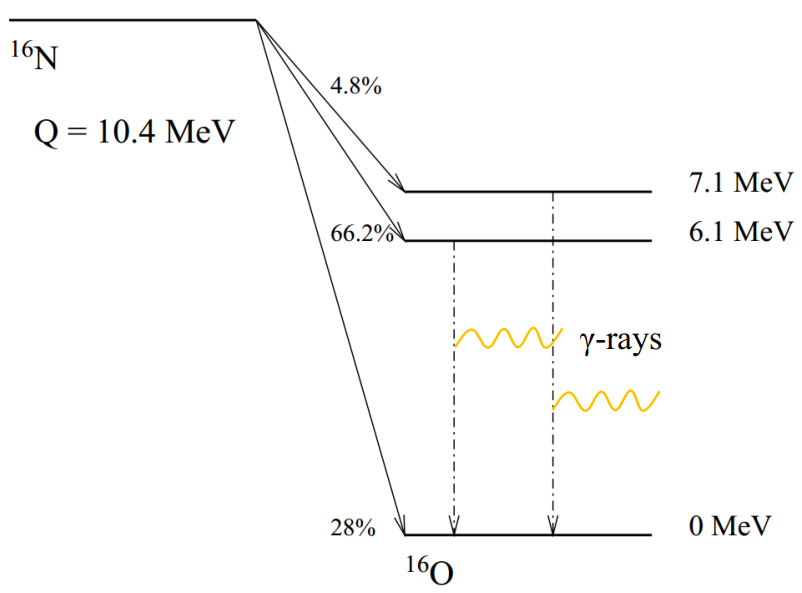
\includegraphics[width=6cm]{n16_decay.png}
	\caption{$^{16}$N main decay scheme, modified from \cite{dragowsky200216n}.}
	\label{n16decay}
\end{figure}


Fig.~\ref{n16pic} shows the geometry of the $^{16}$N source chamber. The chamber is a stainless steel cylinder mainly containing a small PMT and a gas decay chamber. The chamber was designed to confine the electrons from $^{16}$N decay within the chamber and let them be detected by the PMT inside; 


to ensure a high fraction of the $\gamma$-rays 


lighthouse where the liquid in the scintillator volume (for example, pure water in the water phase) is free to enter.


tagged by a small PMT inside

A polyethelene bumper cone is at the bottom of the source.

 



gas capillary tube


 

\cite{dragowsky1999sudbury}.
 

\begin{figure}[!htb]
	\centering
	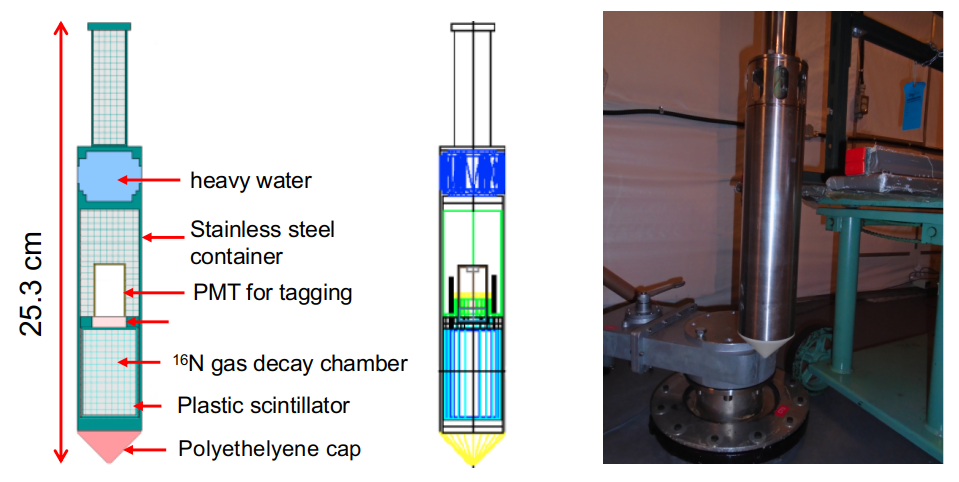
\includegraphics[width=10cm]{n16geom.png}
	\caption{$^{16}$N calibration source geometry. Left: a detailed diagram of $^{16}$N source geometry, modified from \cite{maclellan2009energy,matt_deployedsource}; middle: source geometry implemented in RAT, modified from \cite{n16geom_zach}; right: a picture of the $^{16}N$ source, taken from \cite{n16pic}.}
	\label{n16pic}
\end{figure}



The $^{16}$N calibration runs provide an ideal test of fitter performance. From a comparison of reconstructions for data and MC, we can also extract the resolution and bias of the fitter.



The $\gamma$-rays emitted from the $^{16}$N source interact with the water in the detector mainly via Compton scattering. Figure~\ref{hsx} shows the spatial distributions of the first $\gamma$-ray interaction positions projected on the x axis (called spatial distribution $S(x)$) obtained from MC simulation. The $^{16}$N source is considered as an electron source with a known spatial distribution\cite{boulay2004direct}. For simplicity, in the following we always discuss the $x$ component of the position vector $\vec{X}$. 






\begin{figure}[!htb]
	\centering
	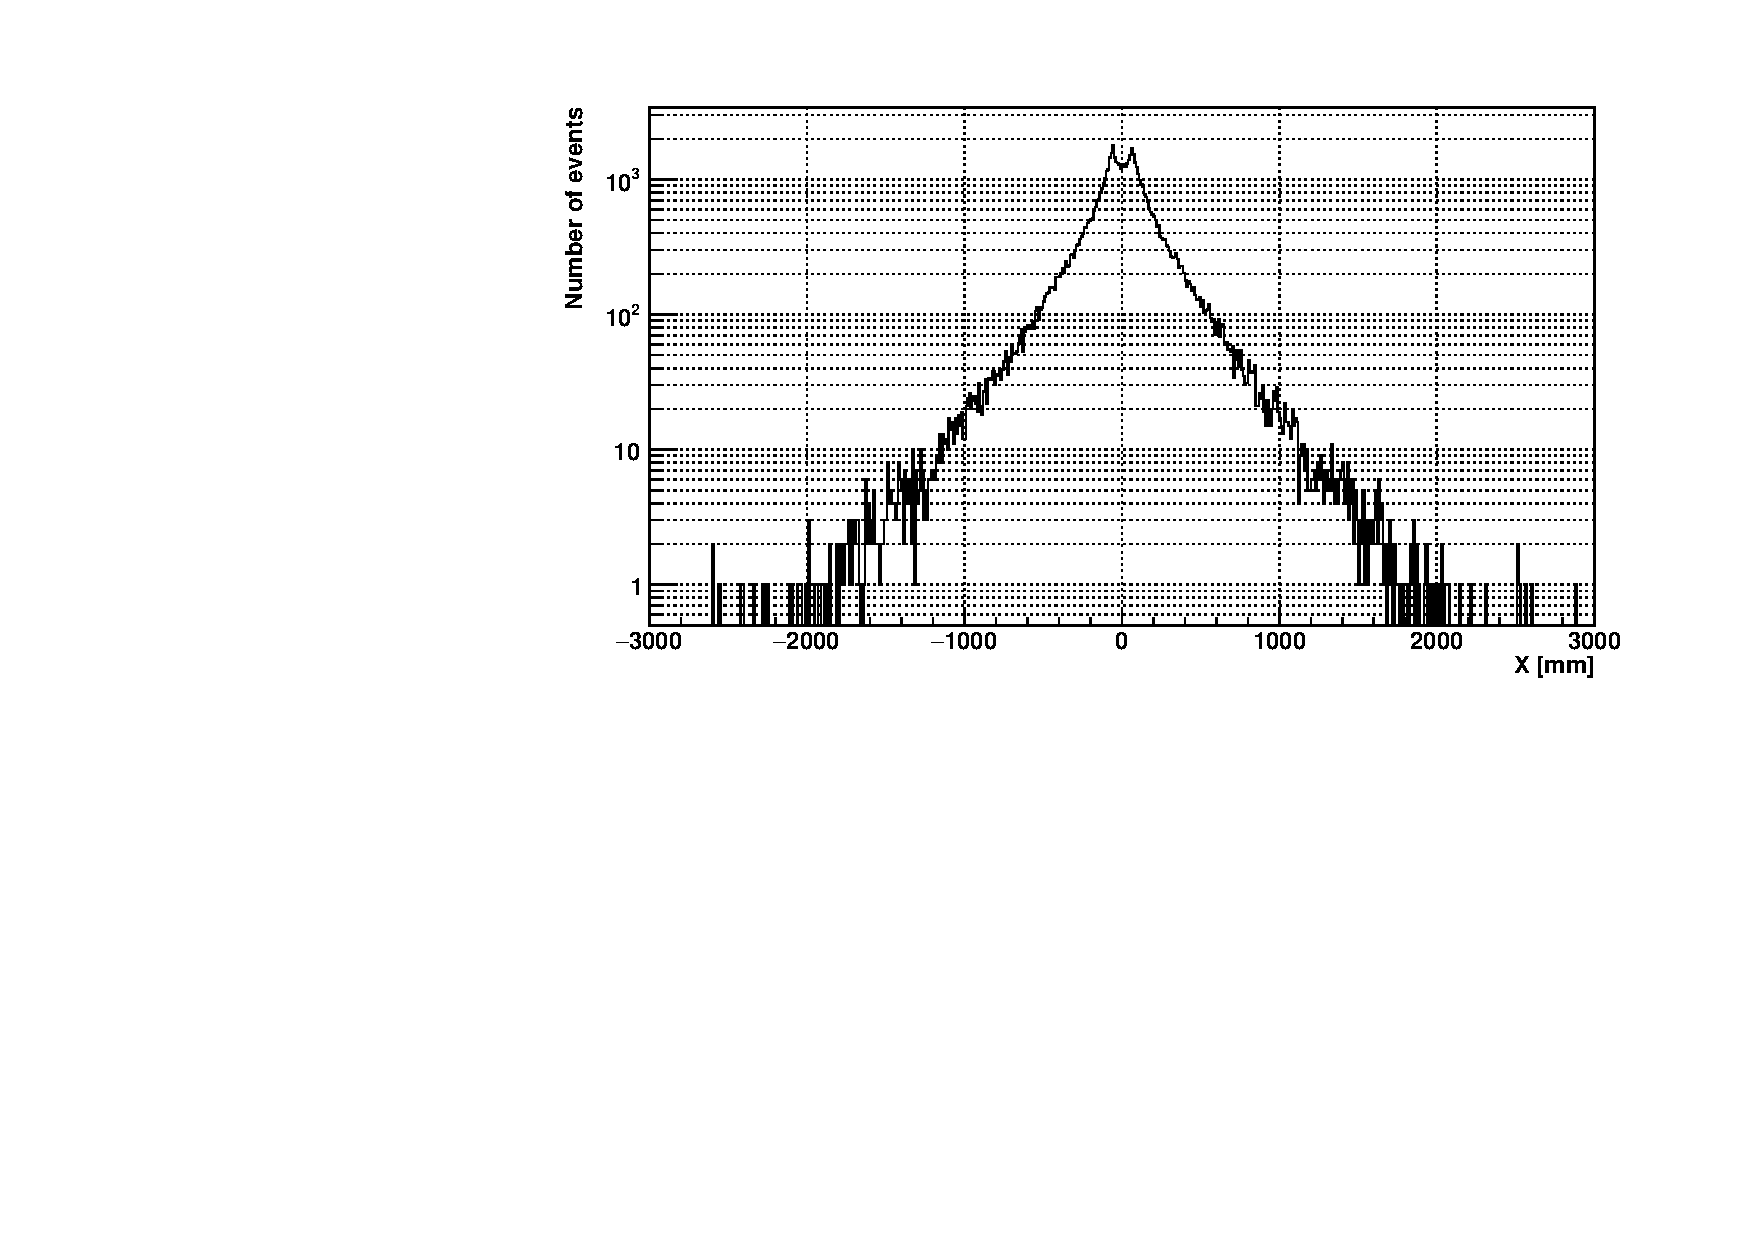
\includegraphics[width=9cm]{sx.pdf}
	\caption{Spatial distributions of {$^{16}$}N first $\gamma$-rays interaction position projected on x axis, obtained from RAT simulations. The double-peak structure is due to the wall of the stainless steel container of the $^{16}N$ source.}
	\label{hsx}
\end{figure}

A position resolution function is defined for the reconstructed electron position distribution\cite{boulay2004direct}:
\[
R(x)=\frac{1-\alpha_e}{\sqrt{2\pi}\sigma_p}\exp{[-\frac{1}{2}(\frac{x-\mu_p}{\sigma_p})^2]+\frac{\alpha_e}{2\tau_p}\exp{[\frac{-|x-\mu_p|}{\tau_p}]}},
\]
where $\alpha_e$ is the fractional exponential component, $\sigma_p$ is
the Gaussian width (corresponding to the position resolution), $\mu_p$ is the Gaussian shift  (corresponding to the position bias) and $\tau_p$ is the exponential slope (corresponding to the position distributions in tails).

For electrons from the $^{16}$N calibration source, their spatial distribution function $N_{R}(x)$ can be described by the position resolution function smeared by the convolution of $S(x)$ as\cite{boulay2004direct}:
\[
N_{R}(x)=\int^{+\infty}_{-\infty} S(x)R(x_{fit}-x)dx.
\]

Since the $S(x)$ and $N_{R}(x)$ are histograms obtained from the data and MC, we calculate by the bin value $x_i$: 
\[N_R(x_i)=\sum_{x_i=-\infty}^{+\infty}S(x_i)R(x_{fit}^i-x_i).\].

The $\chi^2$ is calculated by:
\[
\chi^2=\sum^{N_{bins}}_{i=0}[\frac{N_R(x_{fit}^i)-N_R^{fit}(x_{fit}^i)}{\sigma_i}]^2,
\]
where $N_R^{fit}$ is a trial fit to the $N_R$ by tuning the $\{\alpha_e,\mu_p,\sigma_p,\tau_p\}$ and $\sigma_i$ is taken as the bin width of the histograms.

By minimizing the $\chi^2$, the parameters of the resolution function, $\{\alpha_e,\mu_p,\sigma_p,\tau_p\}$ and a best $N_R^{fit}$ are obtained.

Figure~\ref{posresol} shows a comparison of the reconstructed x position of {$^{16}$}N events between data and MC. The reconstructed position distributions are fitted with $N_R^{fit}$.

%\begin{figure}[!htb]
%	\centering
%	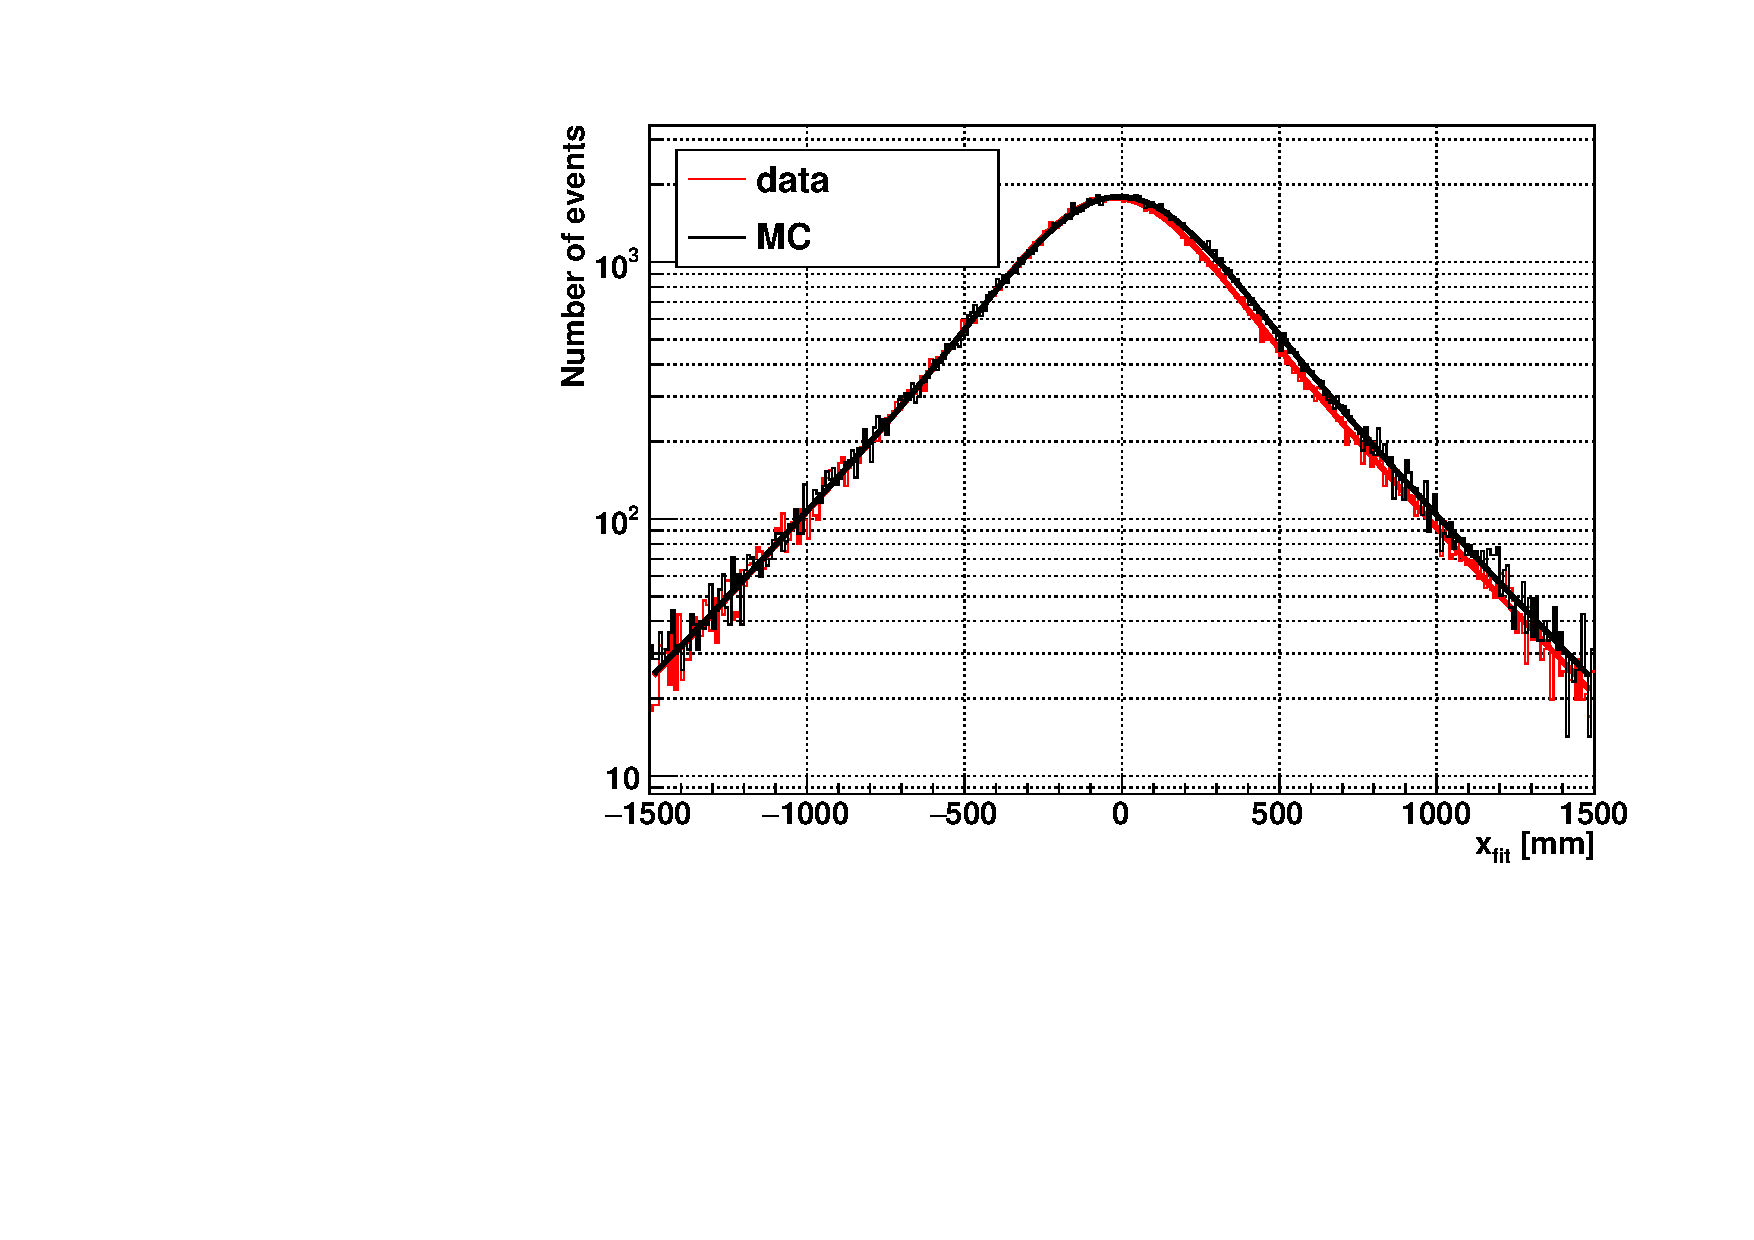
\includegraphics[width=10cm]{posResol.pdf}
%	\caption{Distributions of the reconstructed position projected on x axis, obtained from SNO+ {$^{16}$}N central run data (red) and MC (black). The distributions are fitted with $N_R^{fit}$ (red and black lines).}
%	\label{posresol}
%\end{figure}

Table~\ref{table_posresol} summarizes the values of position resolution parameters obtained from data and MC of {$^{16}$}N calibration runs at the detector center.
\vspace{1mm}
\begin{table}[ht]
	\centering
	\caption{Position resolution parameters for the MP Water Fitter.}
	\label{table_posresol}
	\begin{tabular}{|p{2.5cm}|p{2.2cm}|p{2.1cm}|p{2.1cm}|p{2.1cm}| p{2.1cm}|}
		\hline
		MPW fitter & $\alpha_e$ & $\sigma_P$ (mm) &  $\tau_P$ (mm)& $\mu_P$ (mm)\\
		\hline 
		data& 0.58$\pm$0.04 & 175.8$\pm$3.8 & 288.0$\pm$5.7 & -28.8$\pm$1.0\\	
		\hline 
		MC & 0.51$\pm$0.05 & 195.2$\pm$3.3 & 298.4$\pm$6.1 & -10.9$\pm$1.0\\
		\hline
	\end{tabular}
\end{table}
\vspace{1mm}

Vertex likelihood surface for an typical {$^{16}$}N event (calibration run-100934\_s000\_p001, event GTID = 61836), projected on X-Y, X-Z and Y-Z planes. A clean global maxima gives the reconstructed vertex: the fitted position is at (-211.958, 503.399, 275.990) mm and the fitted time at 217.03885 ns. This is shown in Fig.~\ref{likelihoodSurface}. 

\begin{figure}
	\centering
	%\subfigure[X-Y plane.]{\label{fig:1a}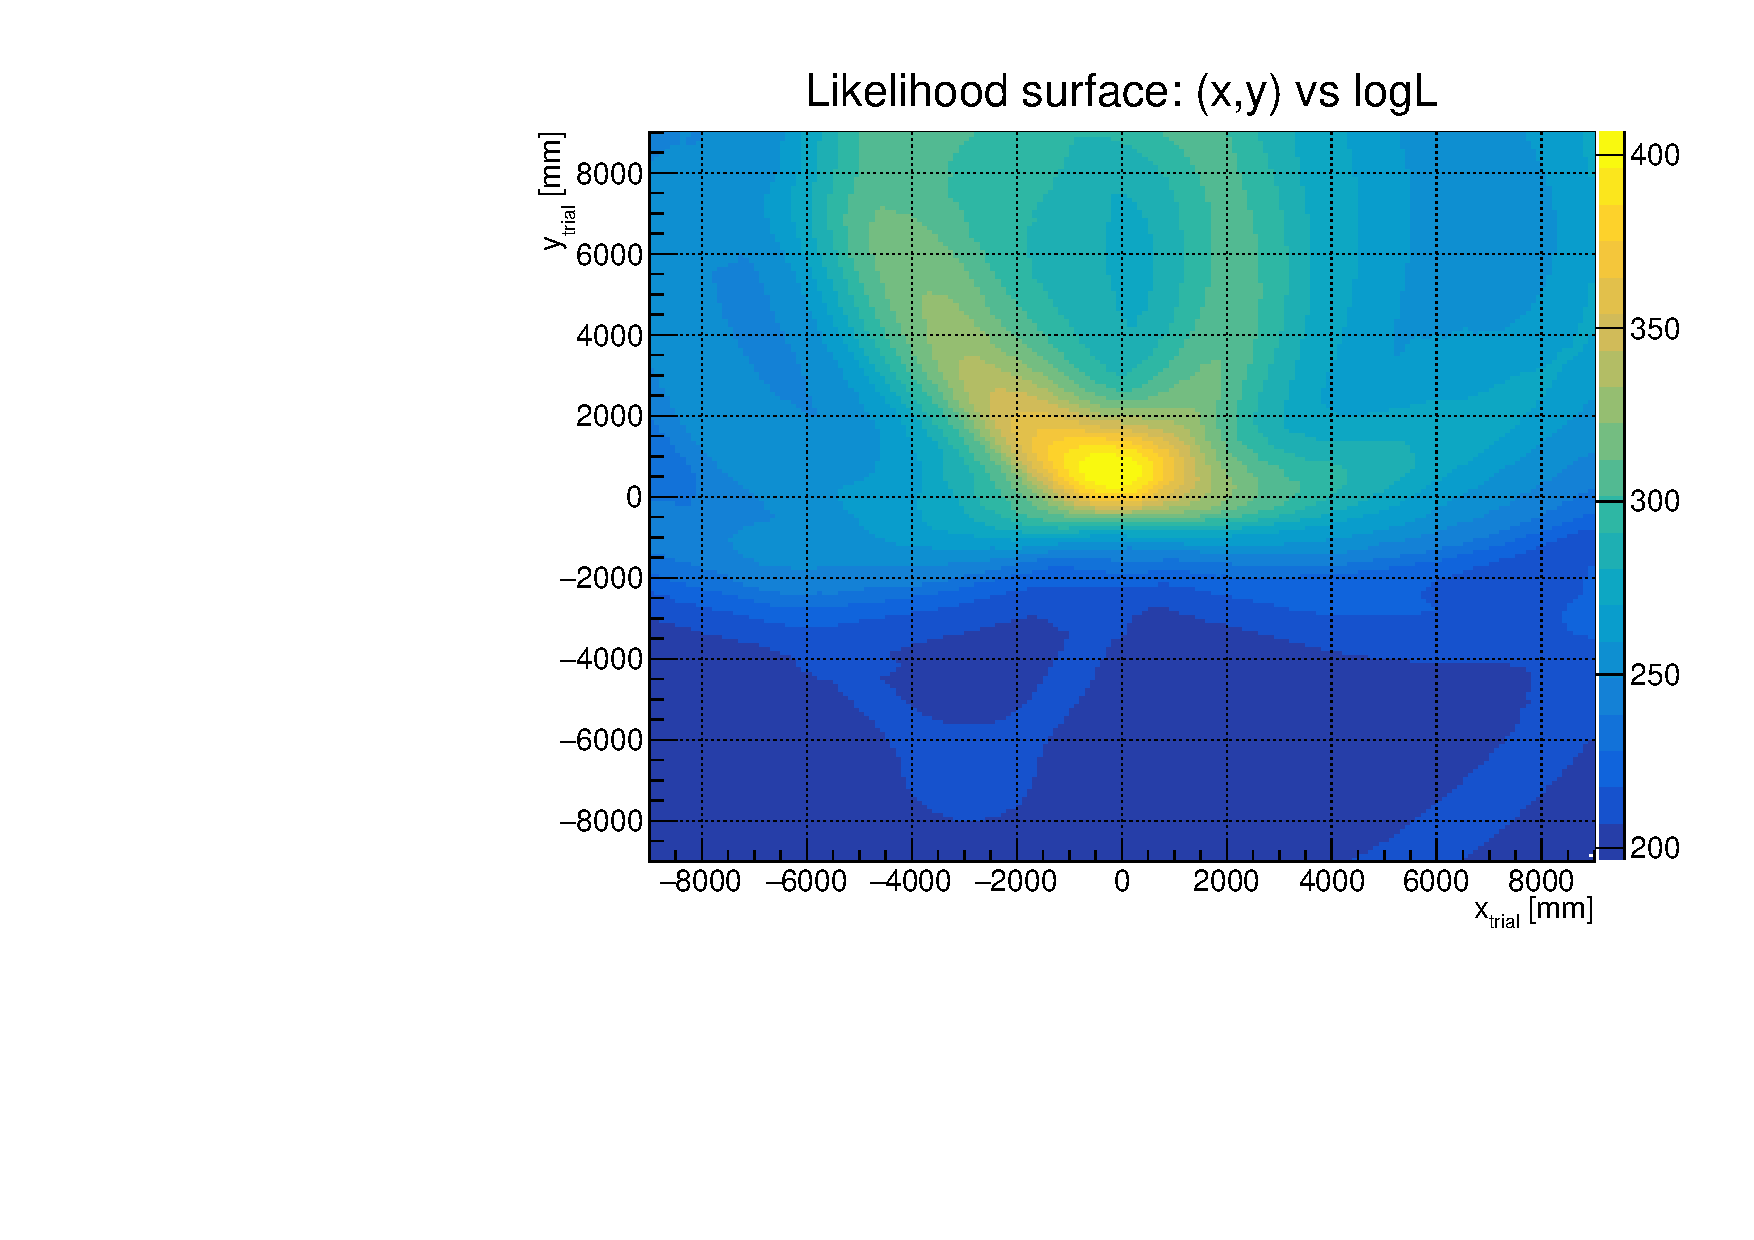
\includegraphics[width=65mm]{likelihoodSurface_xy.pdf}}
	%\subfigure[Y-Z plane.]{\label{fig:1b}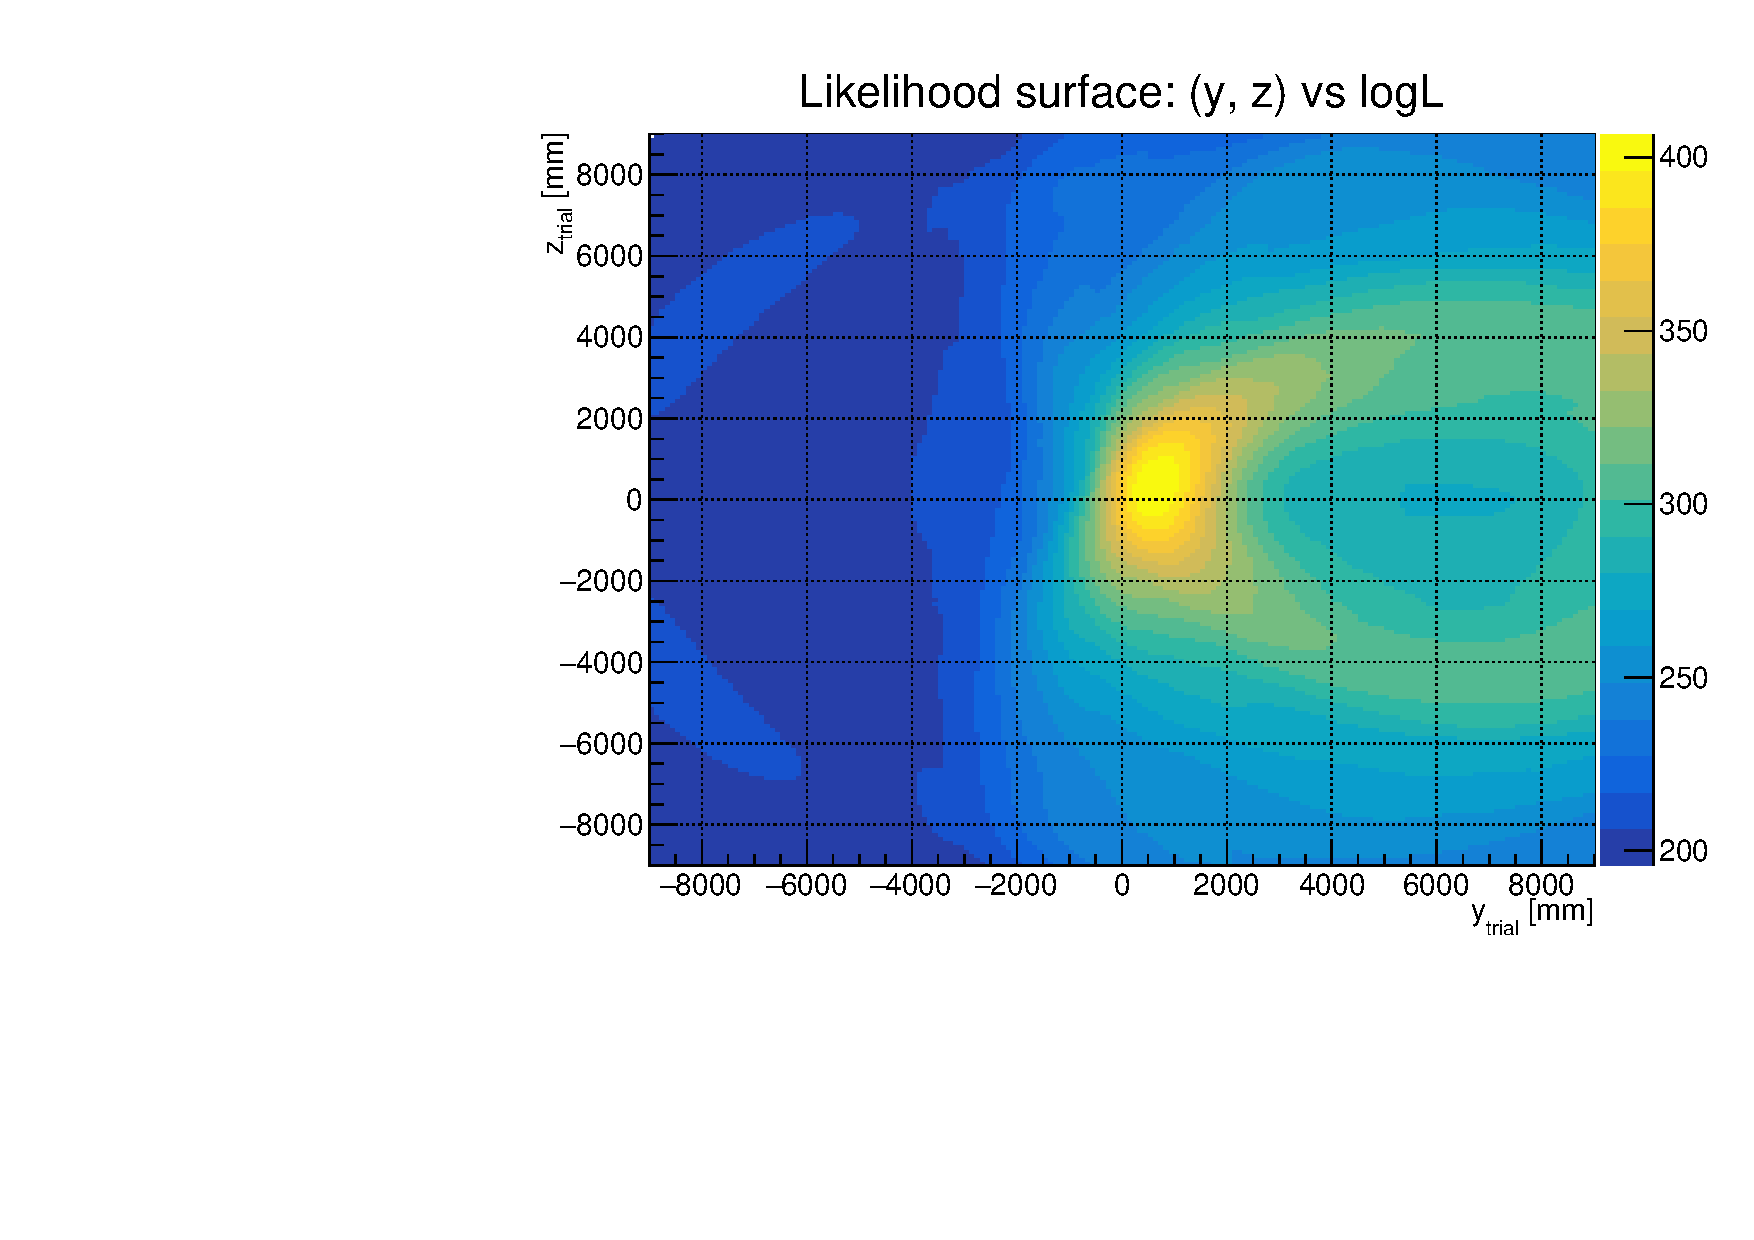
\includegraphics[width=65mm]{likelihoodSurface_yz.pdf}}
	%\subfigure[X-Z plane.]{\label{fig:1c}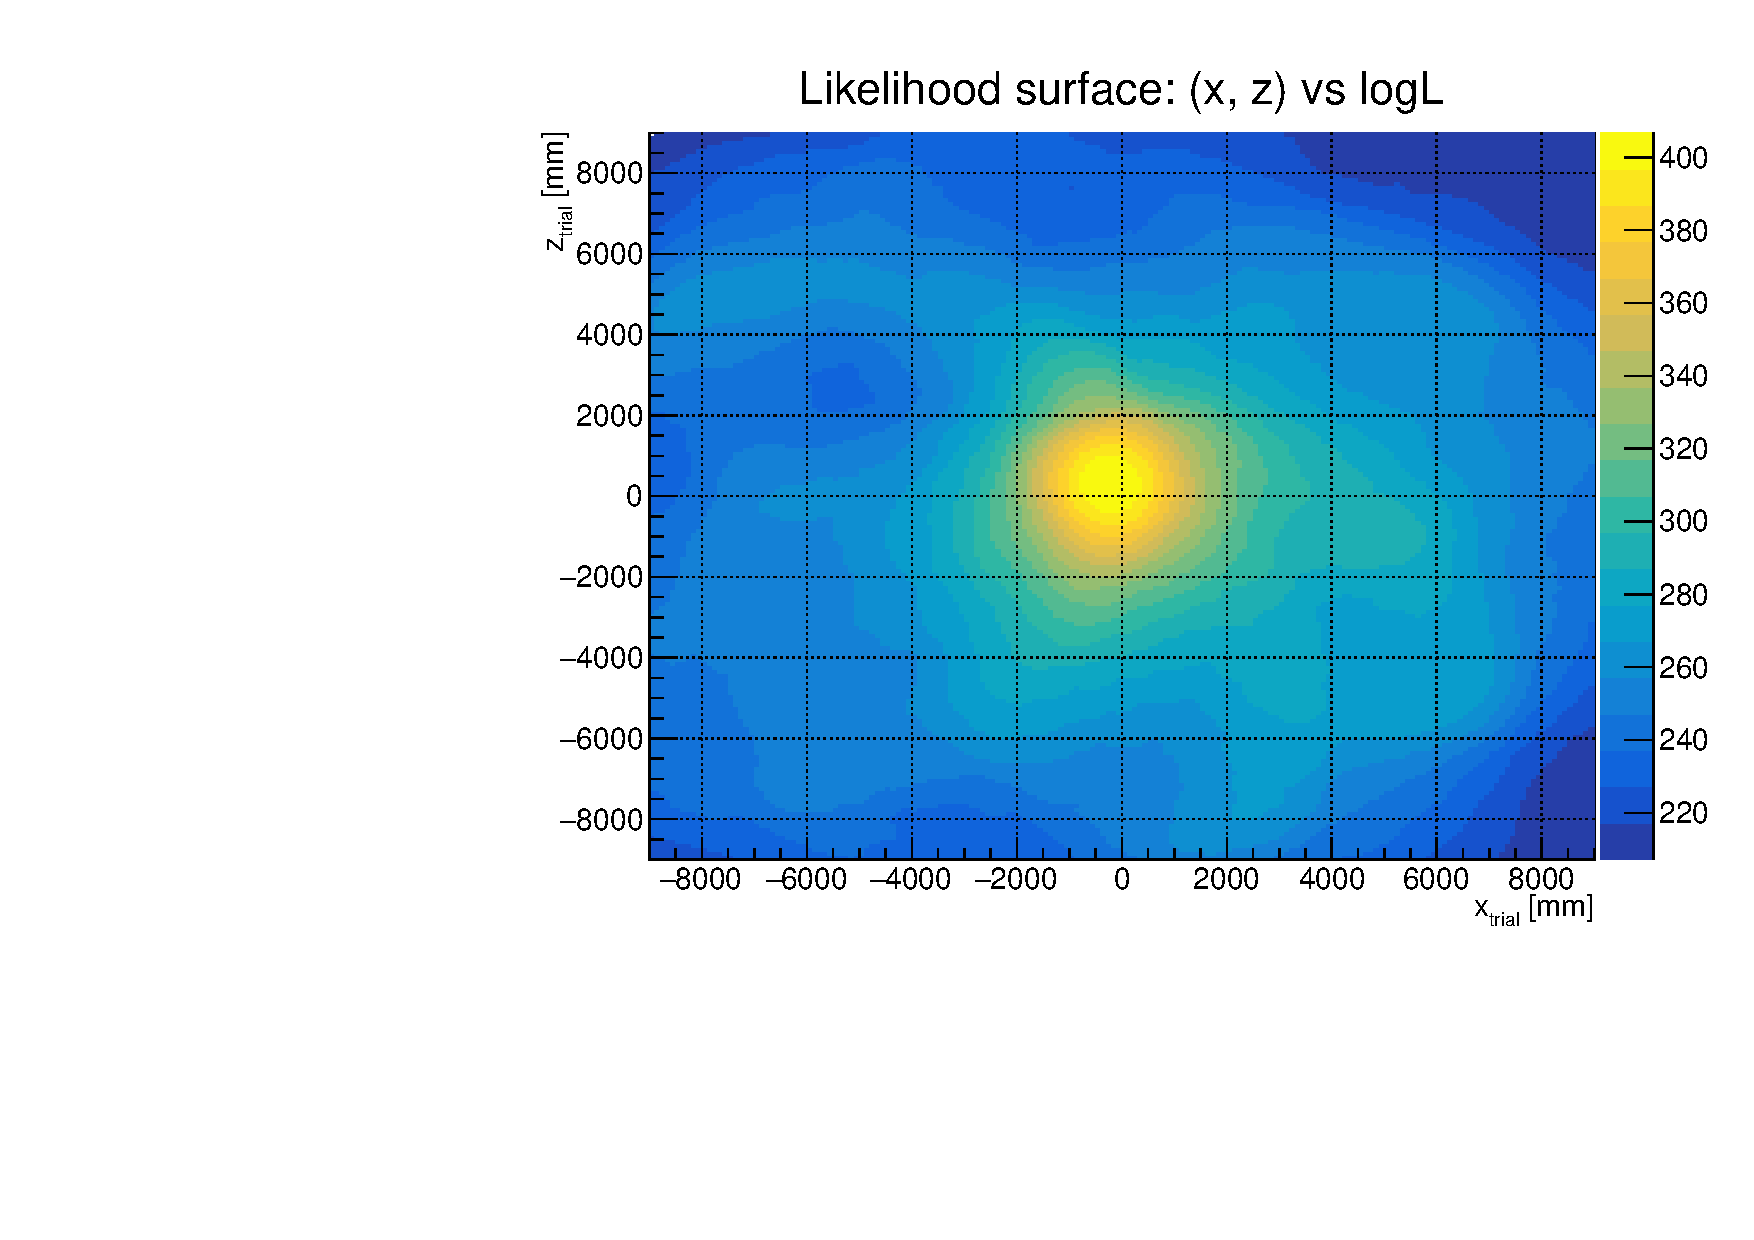
\includegraphics[width=65mm]{likelihoodSurface_xz.pdf}}
	\subfigure[X-Y plane.]{\label{fig:1a}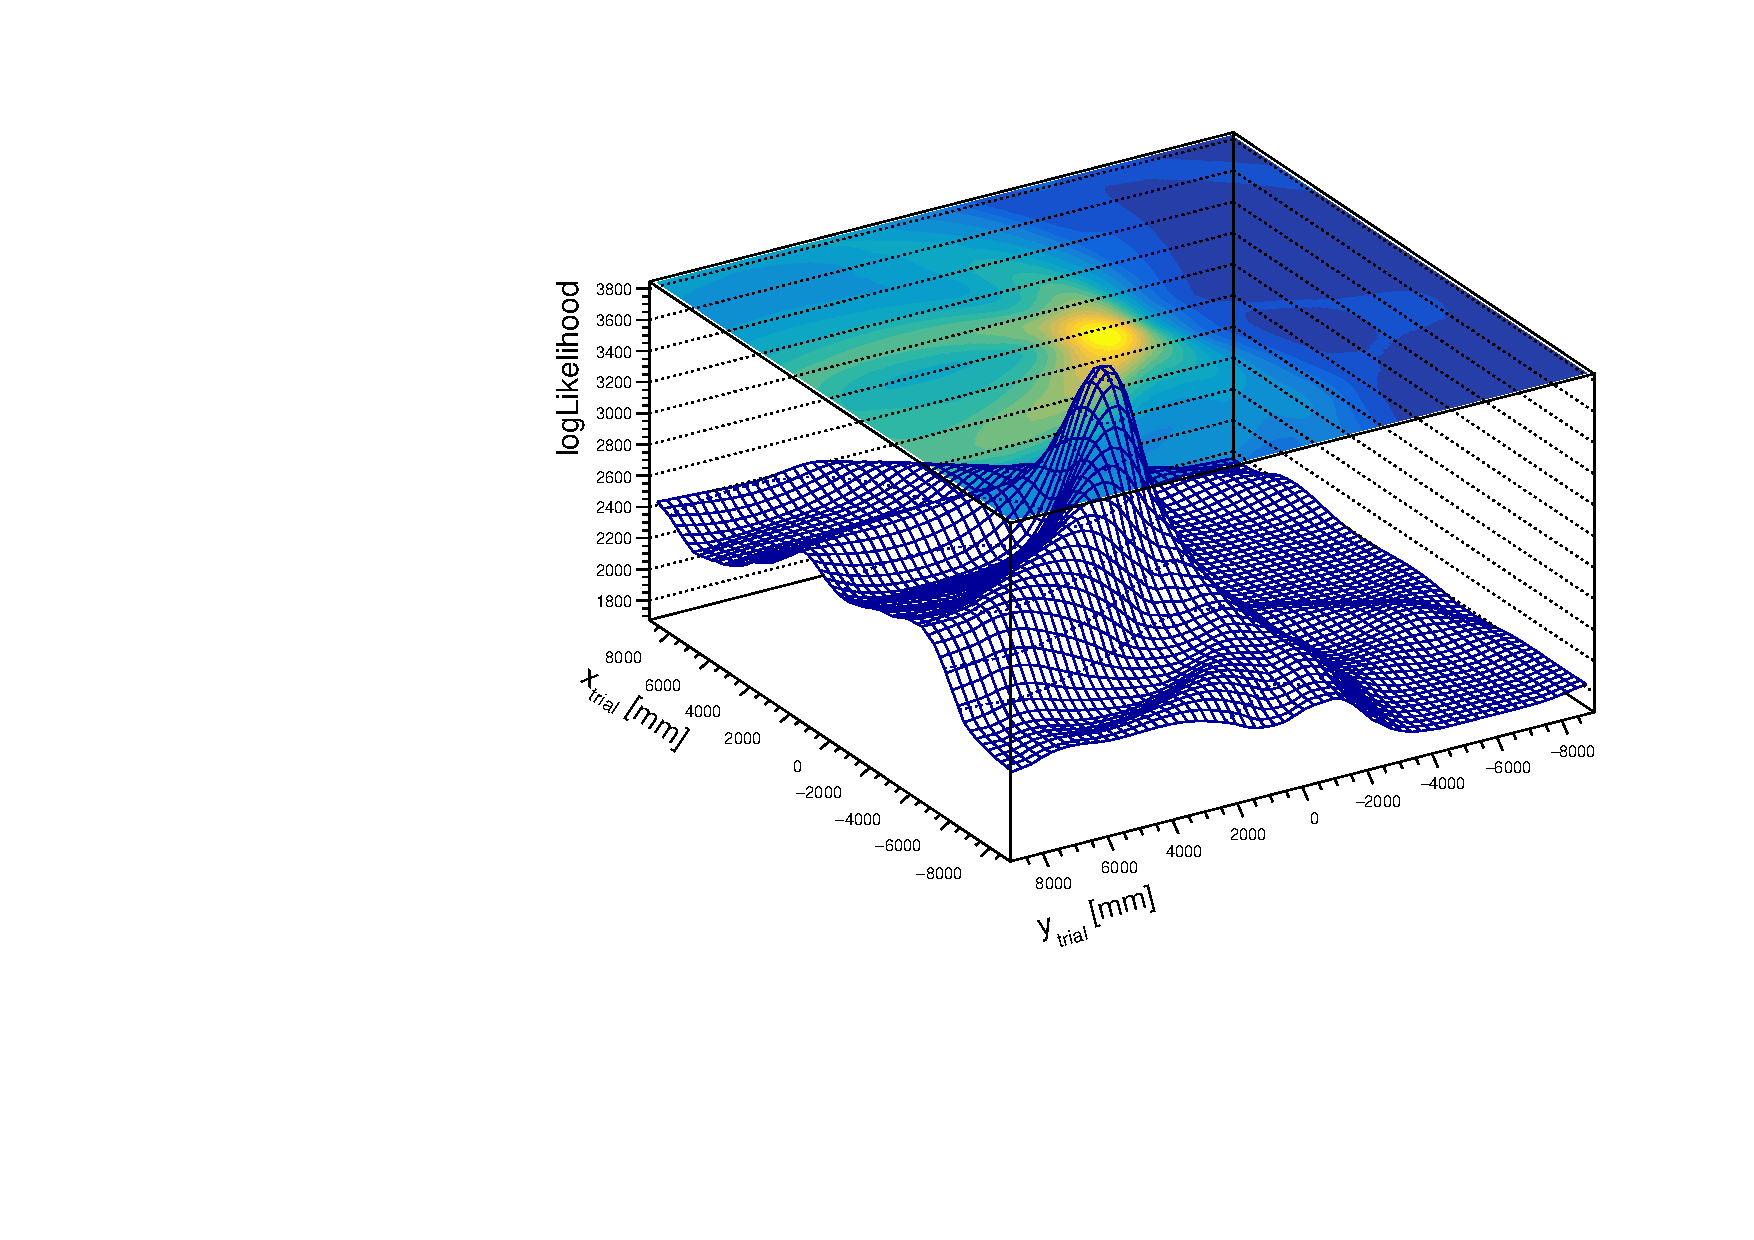
\includegraphics[width=75mm]{surf3_likelihoodXY.pdf}}
	\subfigure[Y-Z plane.]{\label{fig:1b}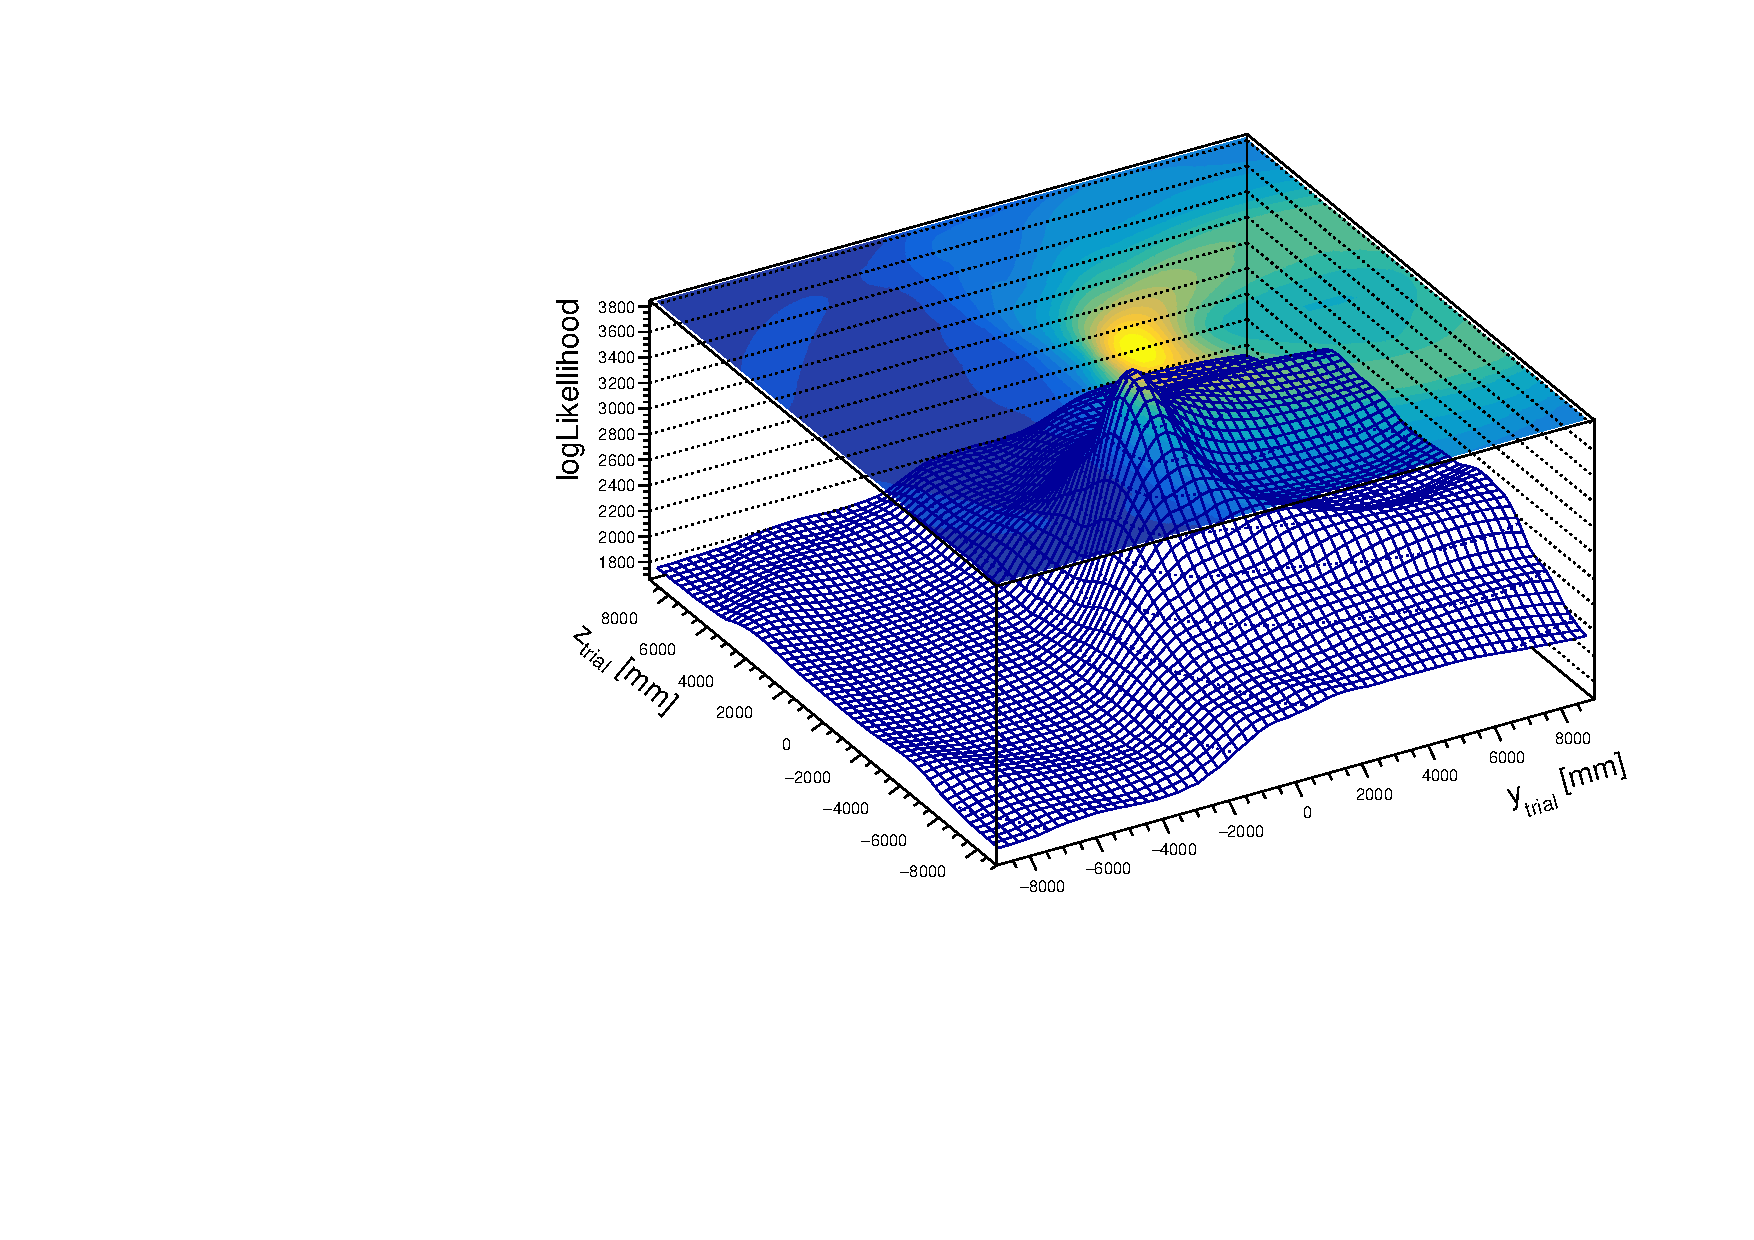
\includegraphics[width=75mm]{surf3_likelihoodYZ.pdf}}
	\subfigure[X-Z plane.]{\label{fig:1c}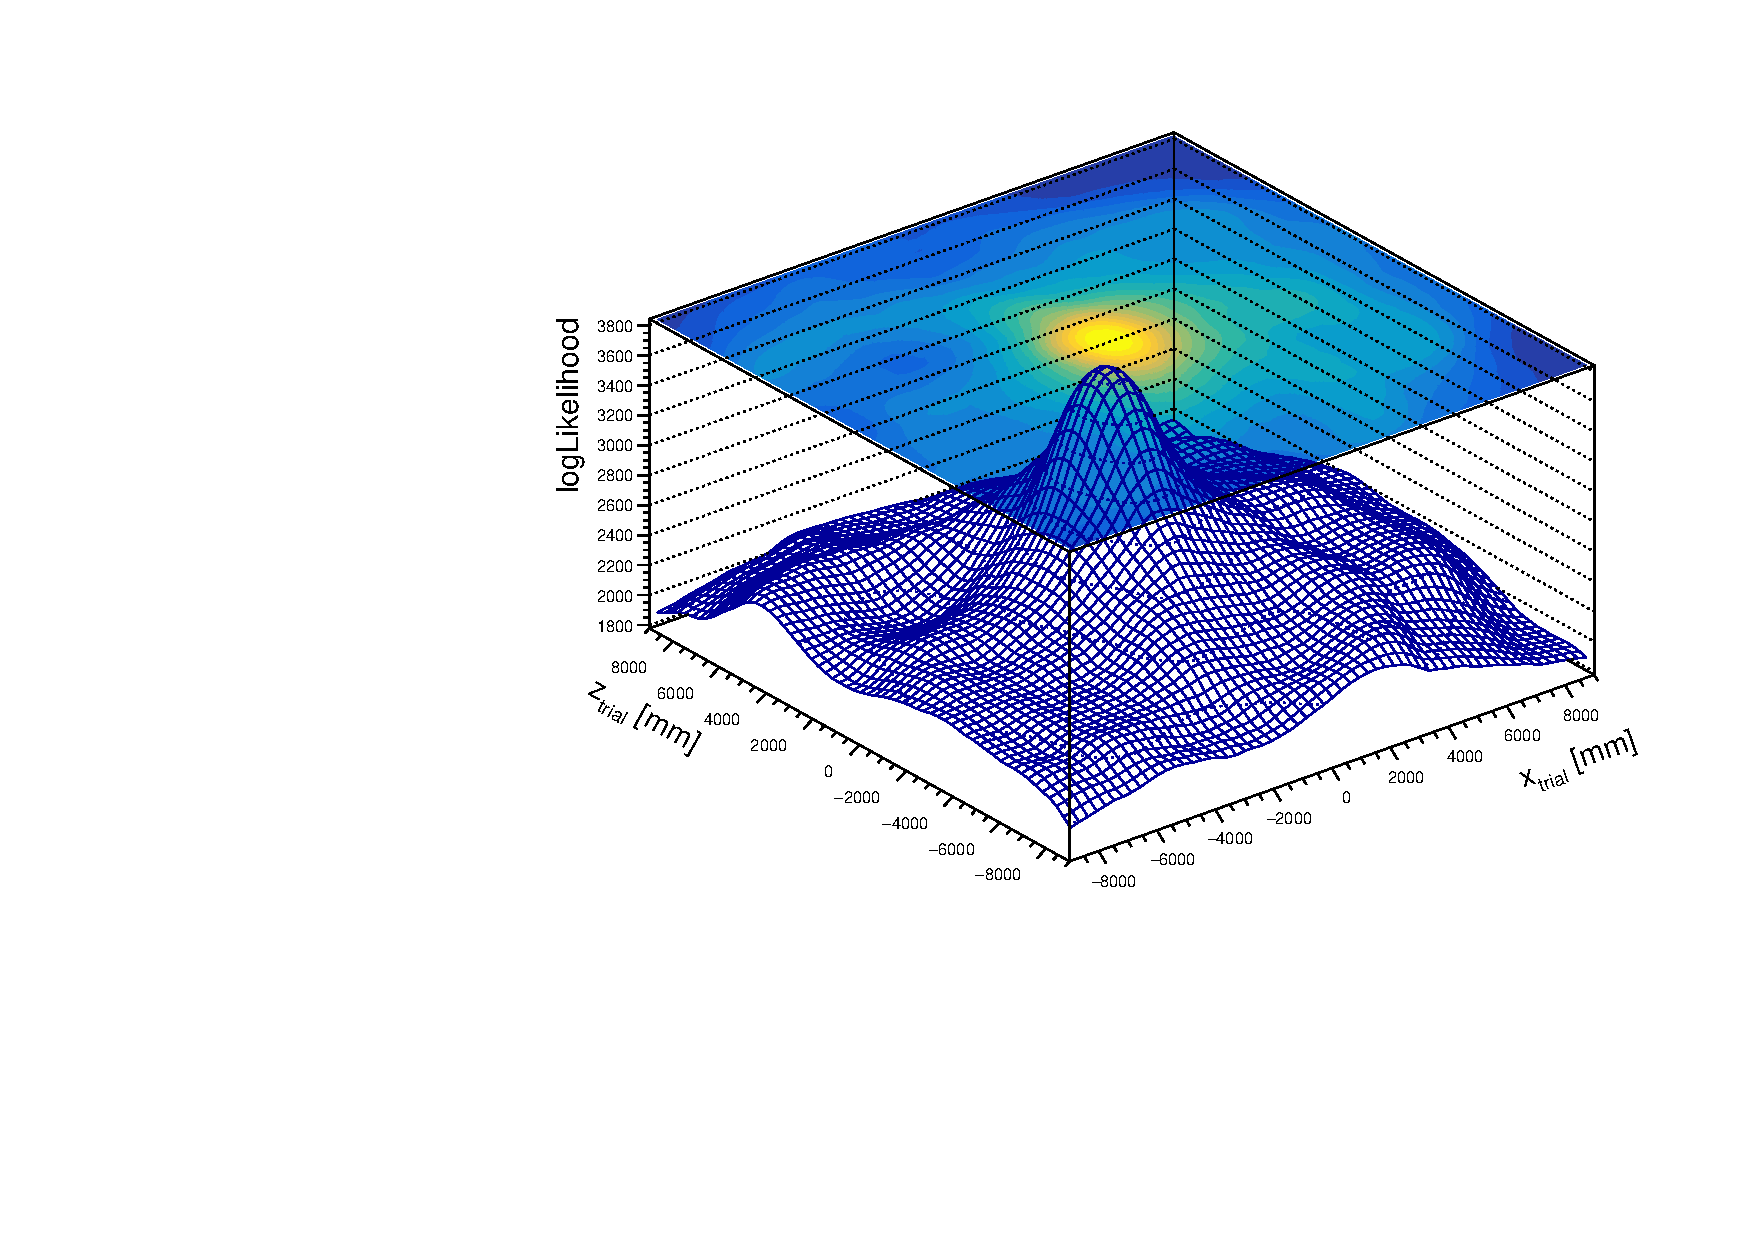
\includegraphics[width=75mm]{surf3_likelihoodXZ.pdf}}
	\caption{Likelihood surface of an {$^{16}$}N event projected on X-Y, Y-Z, X-Z planes. A clear global maxima is reached for the fitted vertex.}
	\label{likelihoodSurface}
\end{figure}


\begin{figure}
	\centering
	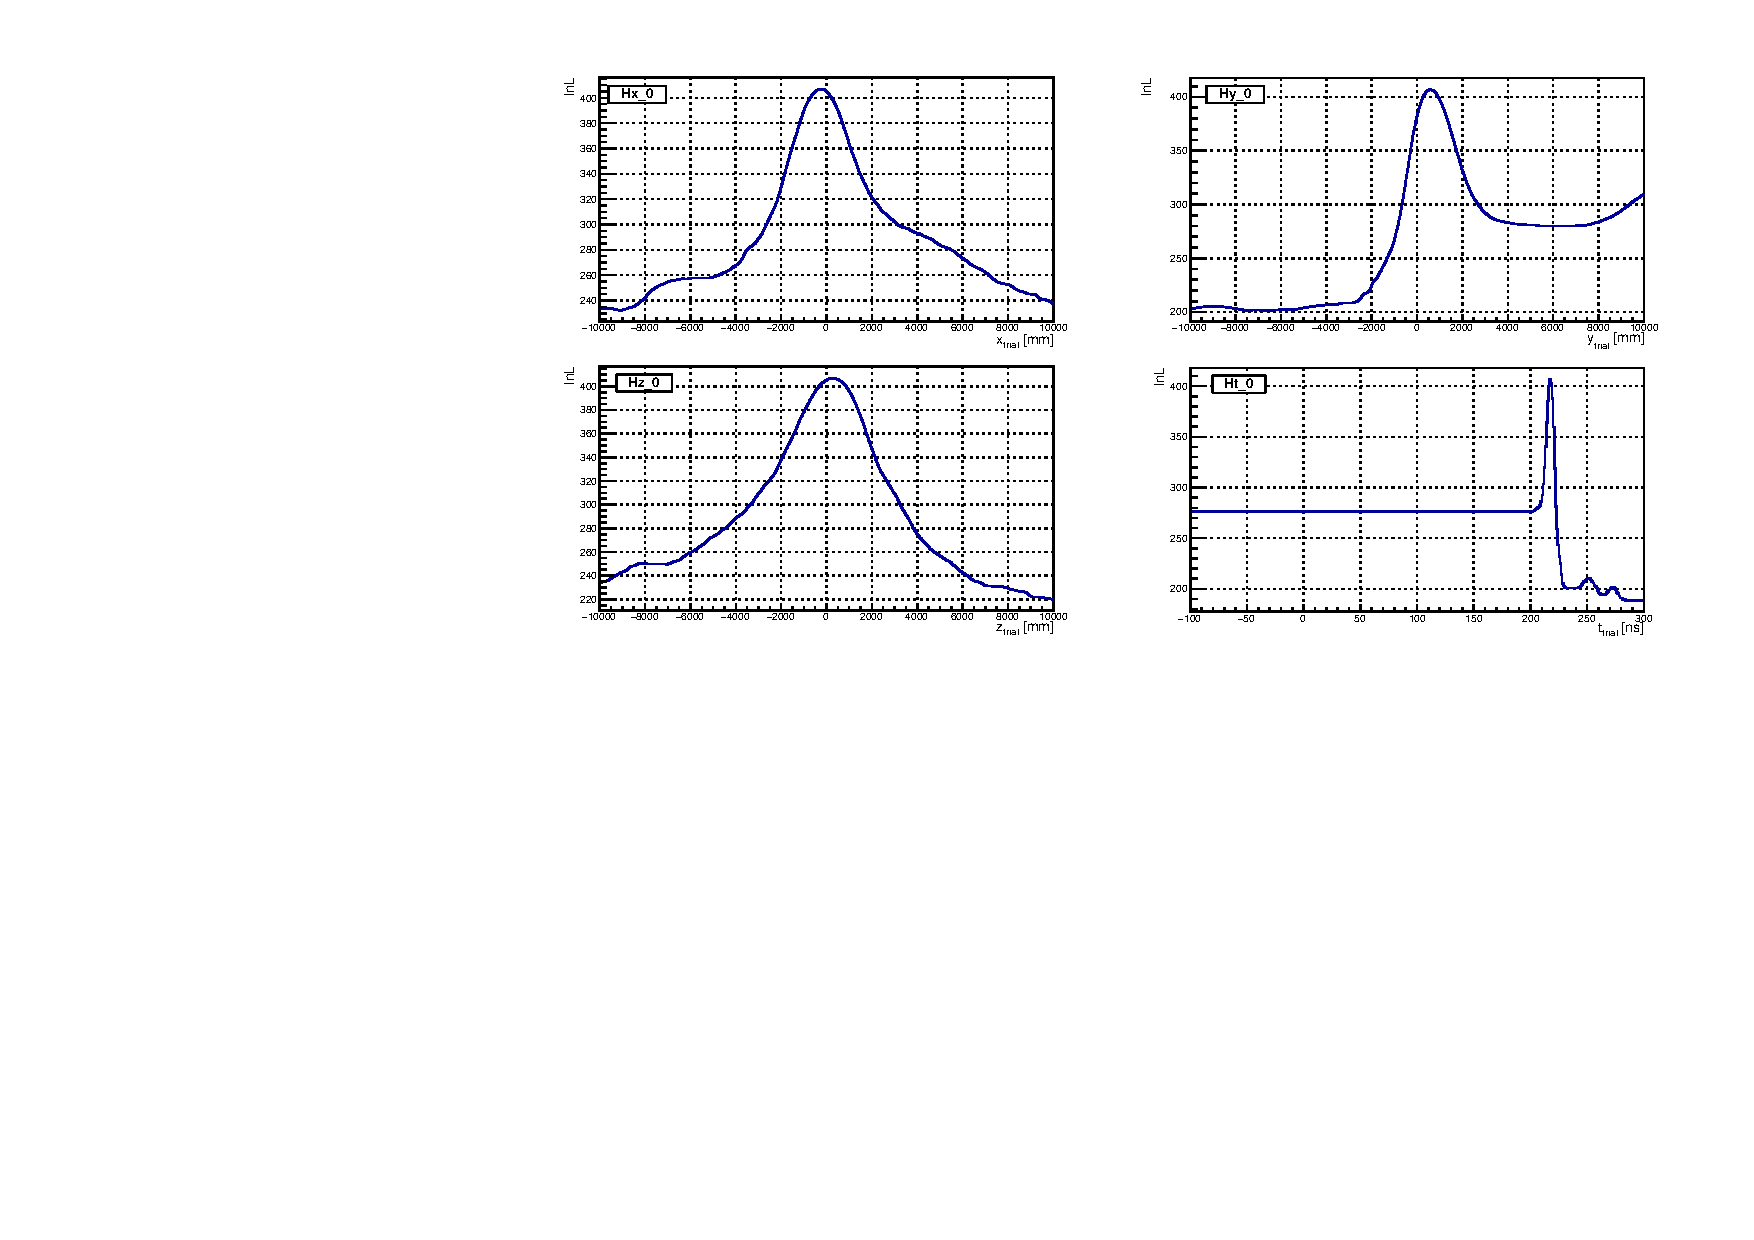
\includegraphics[width=160mm]{logL_xyzt.pdf}
	\caption{Likelihood surface of an {$^{16}$}N event projected on x, y, z, t axes.}
	\label{logLxyz}
\end{figure}

\begin{figure}
	\centering
	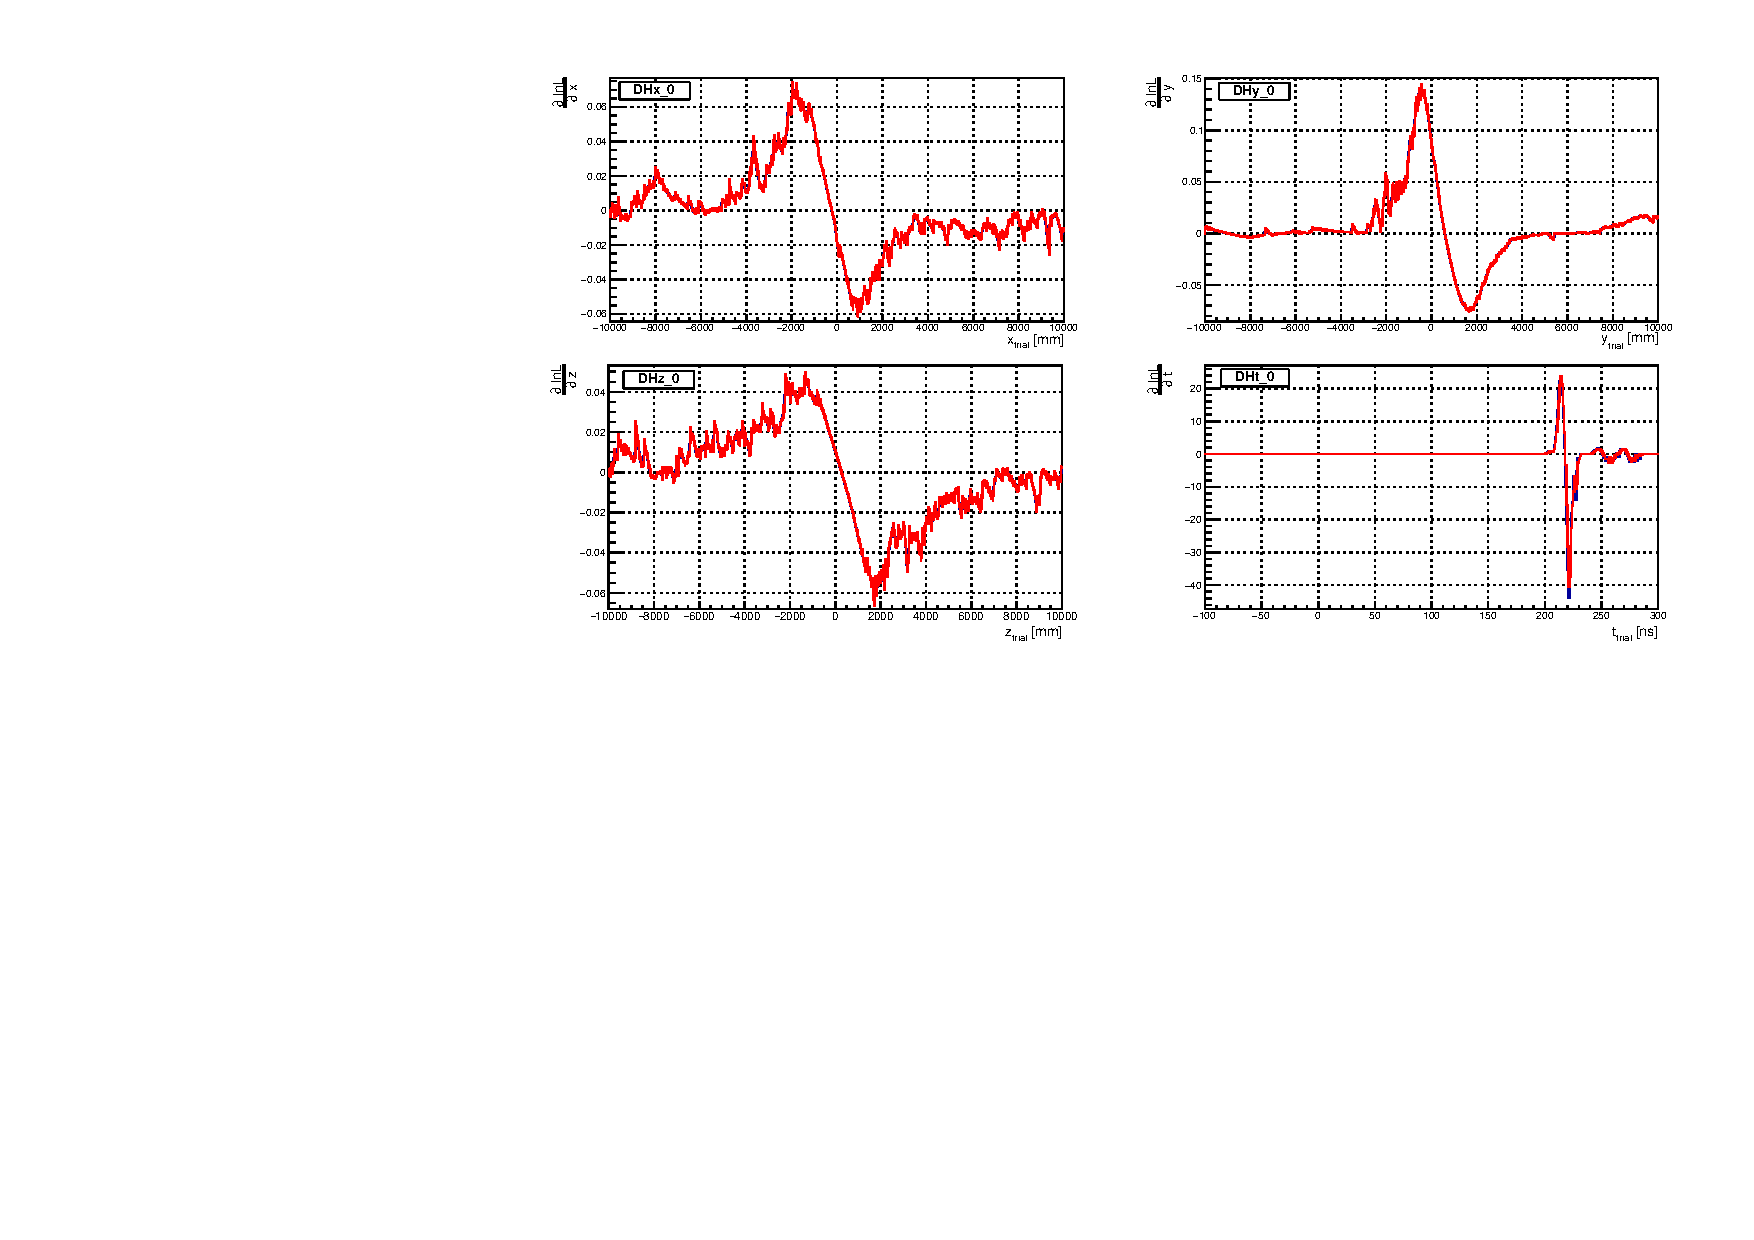
\includegraphics[width=160mm]{derivativeLogL_xyzt.pdf}
	\caption{Derivatives of logLikelihood of an {$^{16}$}N event projected on x, y, z, t axes. The analytical derivatives (blue) are overlaid with numerical derivatives (red). They are well-matched.}
	\label{derivative_logLxyz}
\end{figure}

emit $\gamma$-rays. These $\gamma$-rays will Compton scatter off electrons and the electrons will emit Cherenkov light to be detected by the PMTs.


\subsection{Angular Resolution}
Direction resolutions, with a cut of $|\vec{X}_{fit}-\vec{X}_{src,manip}|>1.5~m$:


Fig.~\ref{angularResolMPW} shows the fits of the angular distributions after $|\vec{X}_{fit}-\vec{X}_{src,manip}|>1.5~m$ cuts.
\begin{figure}
	\centering
	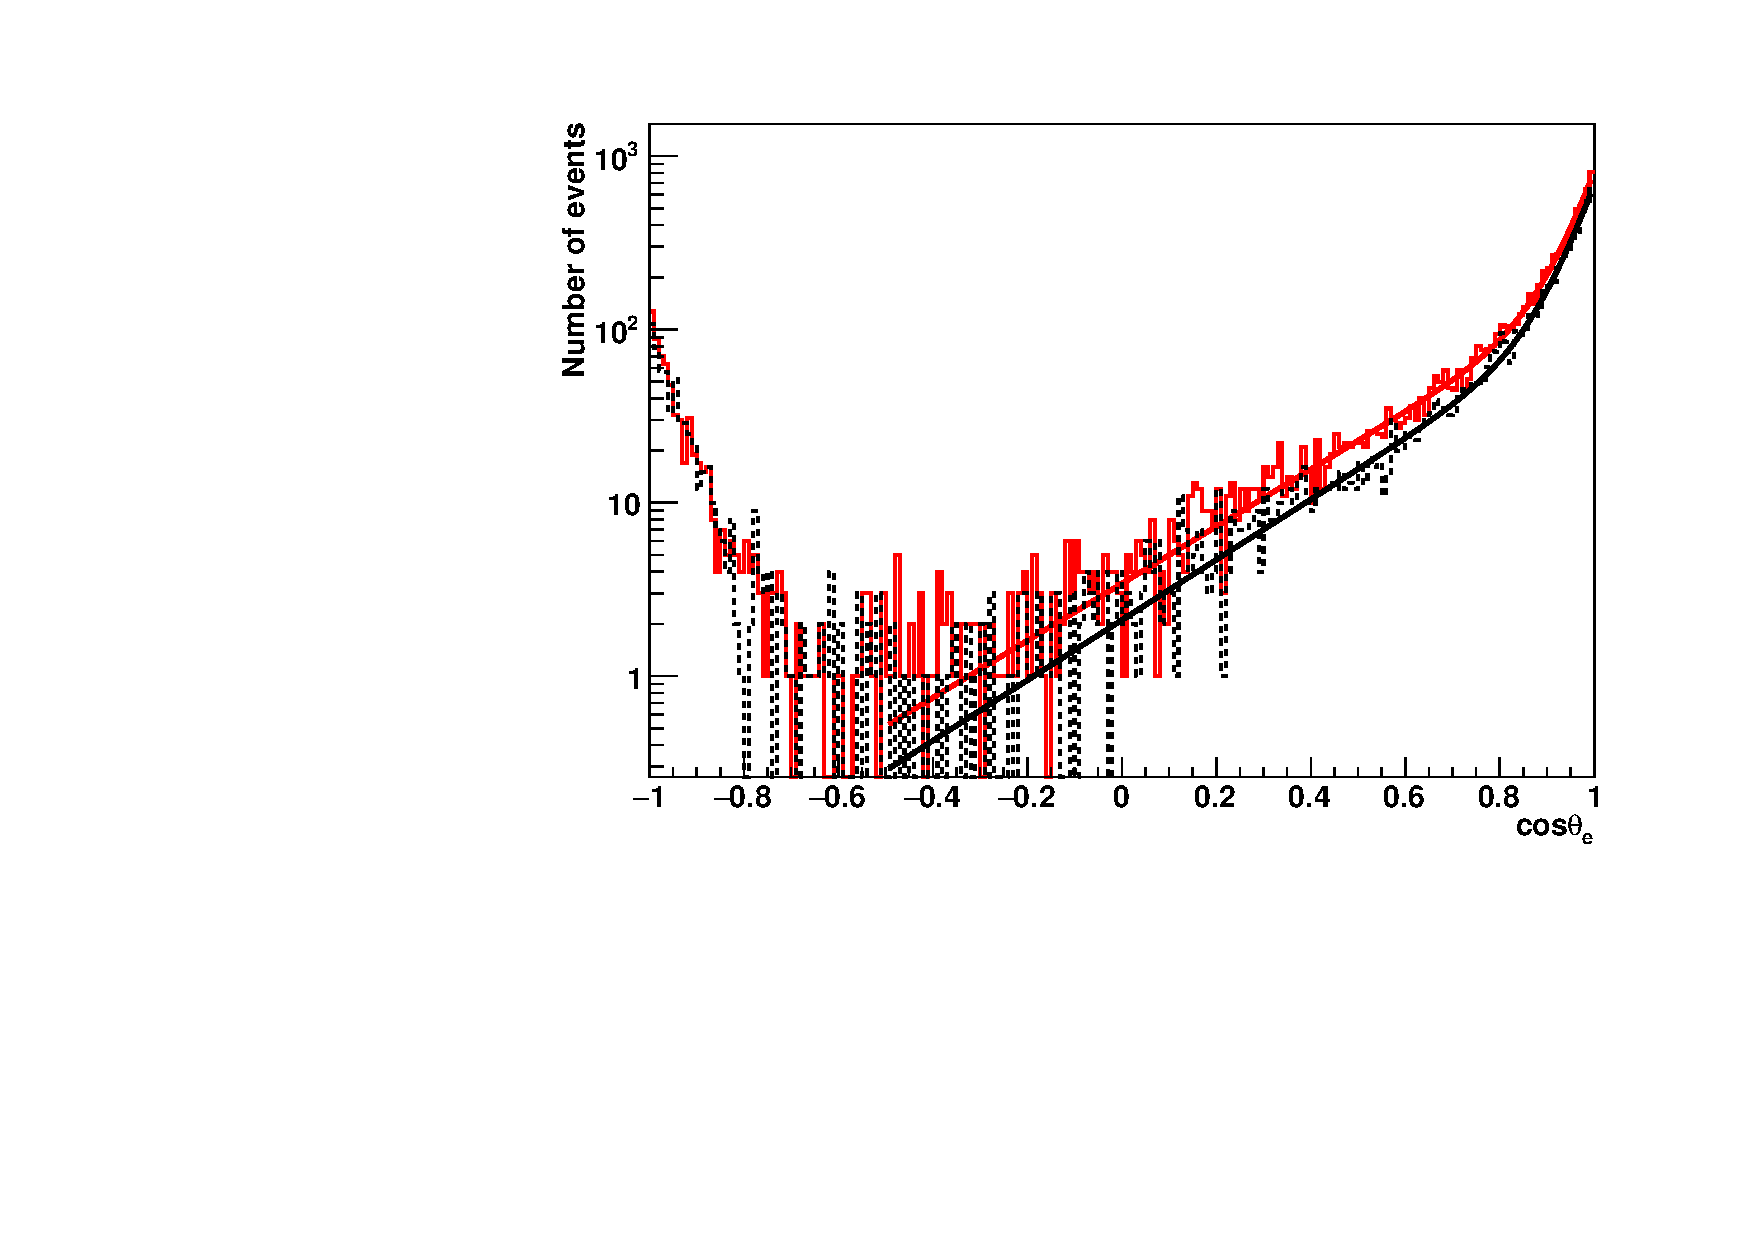
\includegraphics[width=160mm]{angularResol_107055_mpw.pdf}
	\caption{Angular resolutions, compared the data (red solid line) and MC (black dashed line).}
	\label{angularResolMPW}
\end{figure}

The fitted results are shown in Table.~\ref{angularResolValues}.
\begin{table}[ht]
\begin{tabular}{|p{2.2cm}|p{1.8cm}|p{2cm}|p{2cm}|p{1.8cm}|p{1.1cm}|p{1.1cm}|p{1.1cm}| }
	\hline
	107055& $\beta_M$ &  $\beta_S$ & $\alpha_M$ & $\chi^2$/ndf & $\cos\theta_{0.5}$ & $\cos\theta_{0.8}$& $\cos\theta_{0.9}$\\
	\hline
	Rat data & 3.50$\pm$0.11 & 18.48$\pm$0.82 & 0.51$\pm$0.02 & 127.8/140 & 0.991 & 0.733 & 0.338\\
	Rat MC  & 3.74$\pm$0.15 & 19.58$\pm$0.92 & 0.48$\pm$0.02 & 137.1/138 & 1 & 0.768 & 0.398\\	
	\hline
	MPW data & 3.79$\pm$0.12 & 18.58$\pm$0.95 & 0.53$\pm$0.02 & 154.6/143 & 0.982 & 0.743 & 0.379\\
	MPW MC &4.01$\pm$0.19 & 18.41$\pm$1.06 & 0.48$\pm$0.03 & 128.4/127 & 1 & 0.779 & 0.433  \\
	\hline
\end{tabular}
\label{angularResolValues}
\end{table}


\section{Solar $\nu_e$ Analysis and Background Separation in Water Phase}


solar neutrino candidate events in the open dataset.

\begin{figure}[htbp]
	\centering
	\subfigure[Run 100093, GTID 11108354]{ 
		\begin{minipage}[t]{0.4\textwidth}
			\centering
			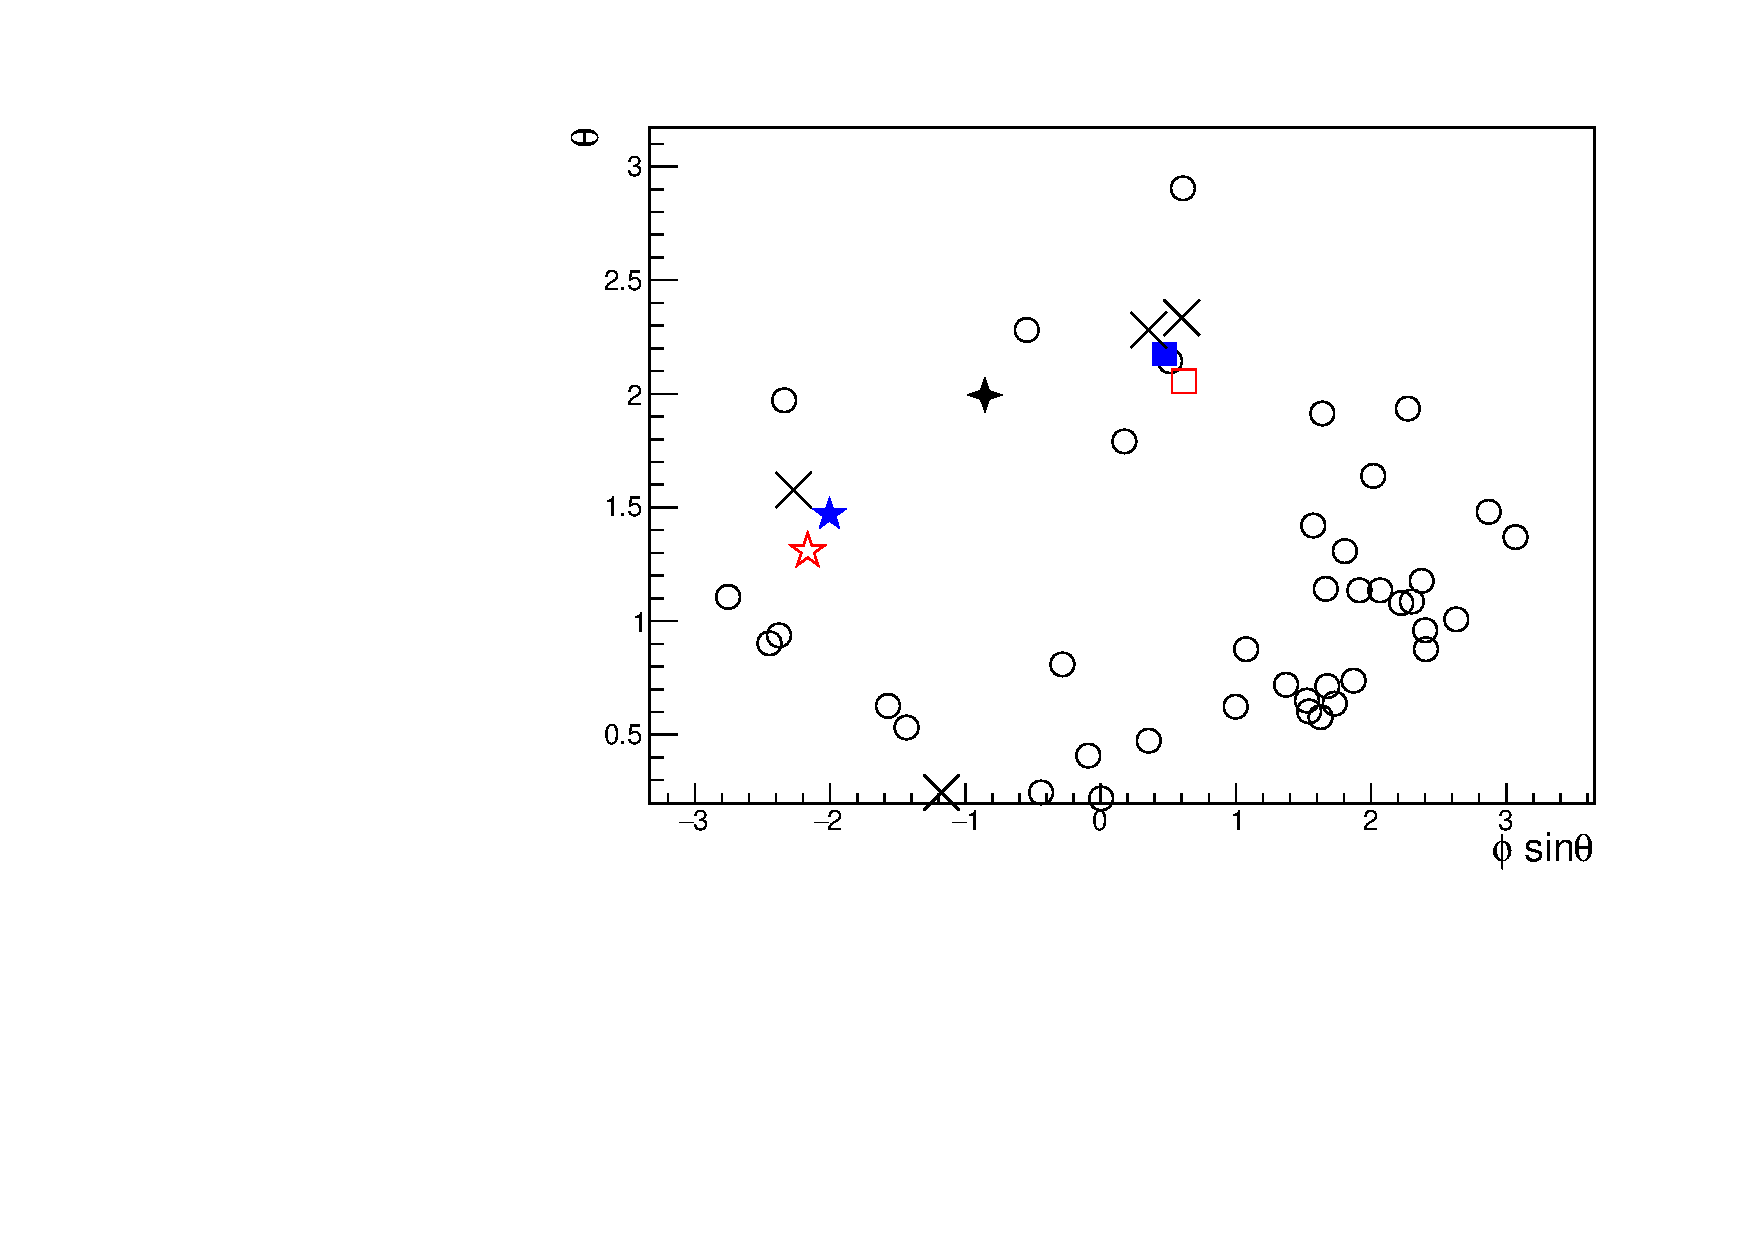
\includegraphics[width=6cm]{PMTmap_100093.pdf}
		\end{minipage}
	}
	\subfigure[Run 100207, GTID 5079885]{ 
		\begin{minipage}[b]{0.4\textwidth}
			\centering
			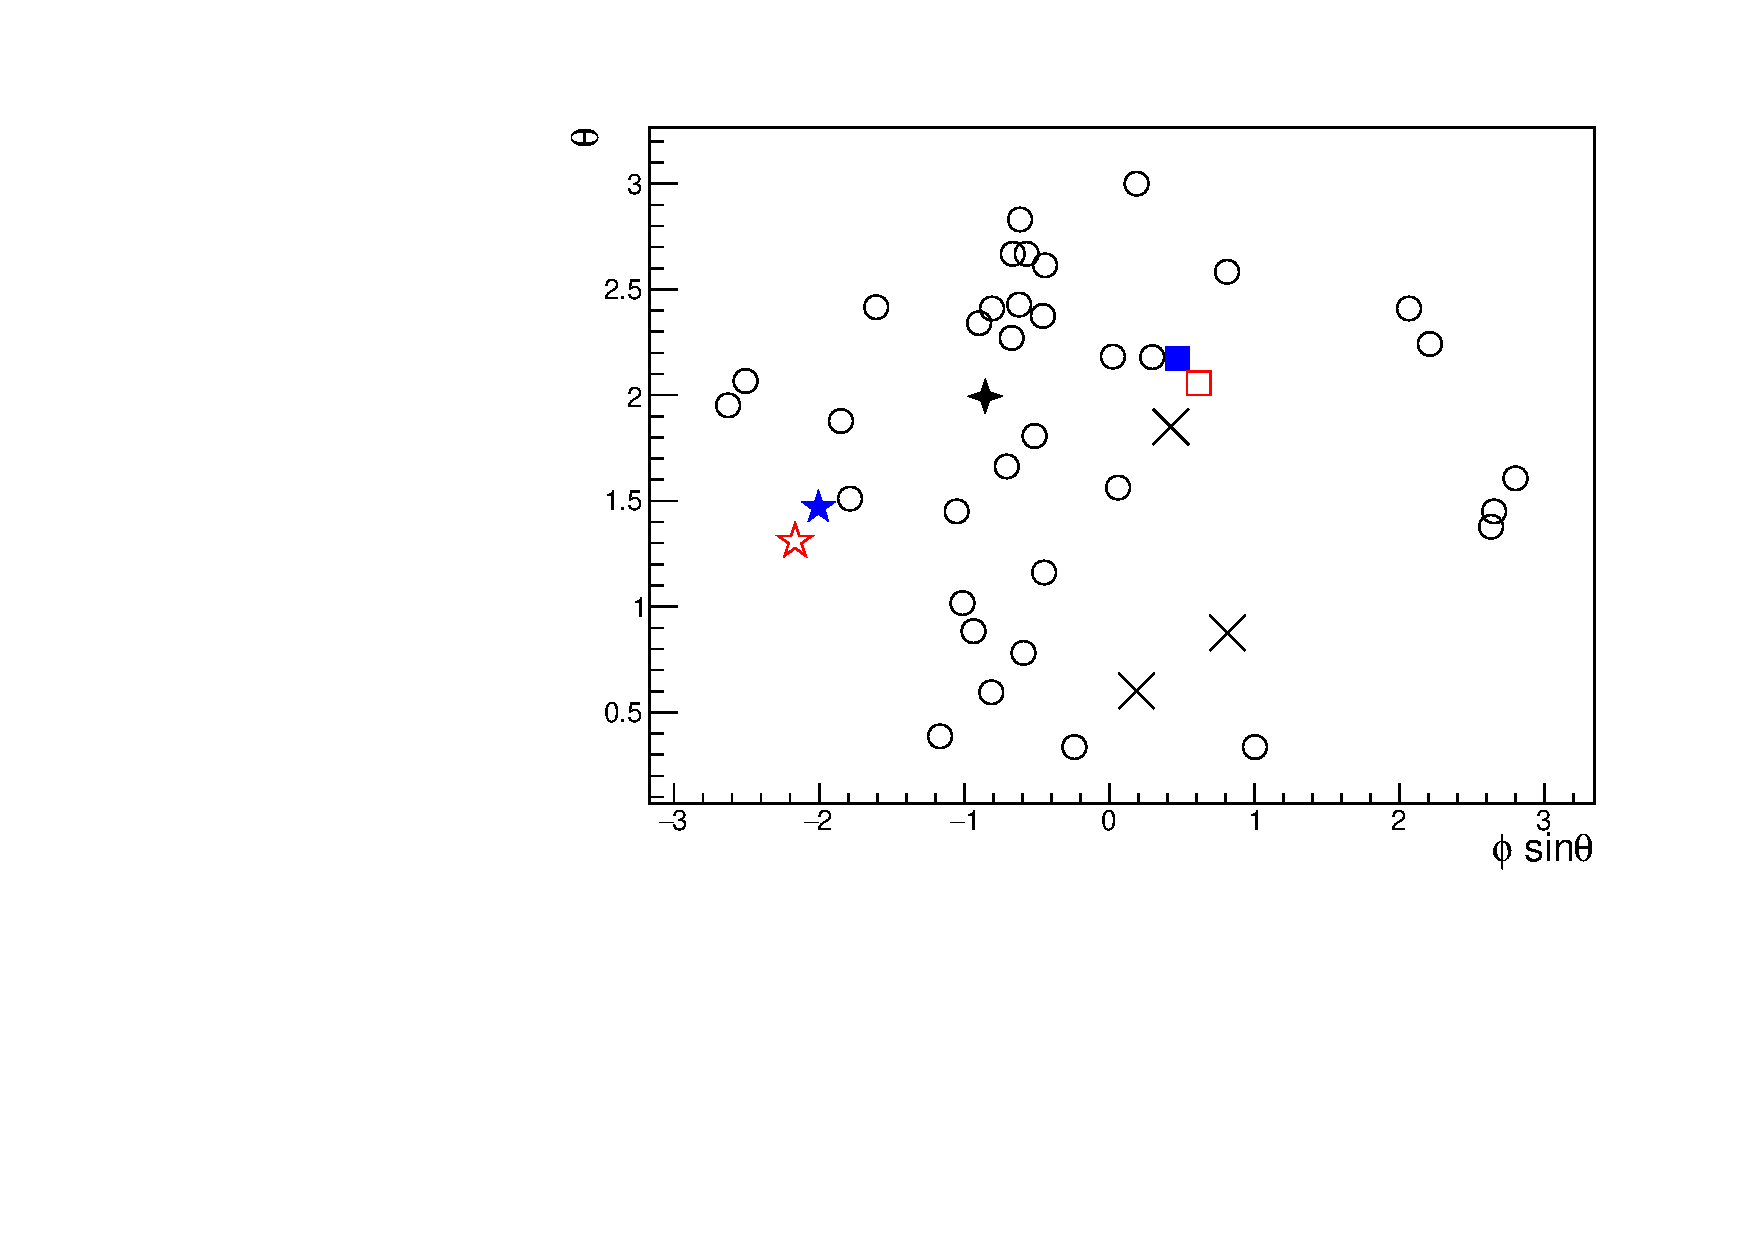
\includegraphics[width=6cm]{PMTmap_100207.pdf}
		\end{minipage}
	}
	\subfigure[Run 100632, GTID 7882360]{ 
		\begin{minipage}[t]{0.4\textwidth}
			\centering
			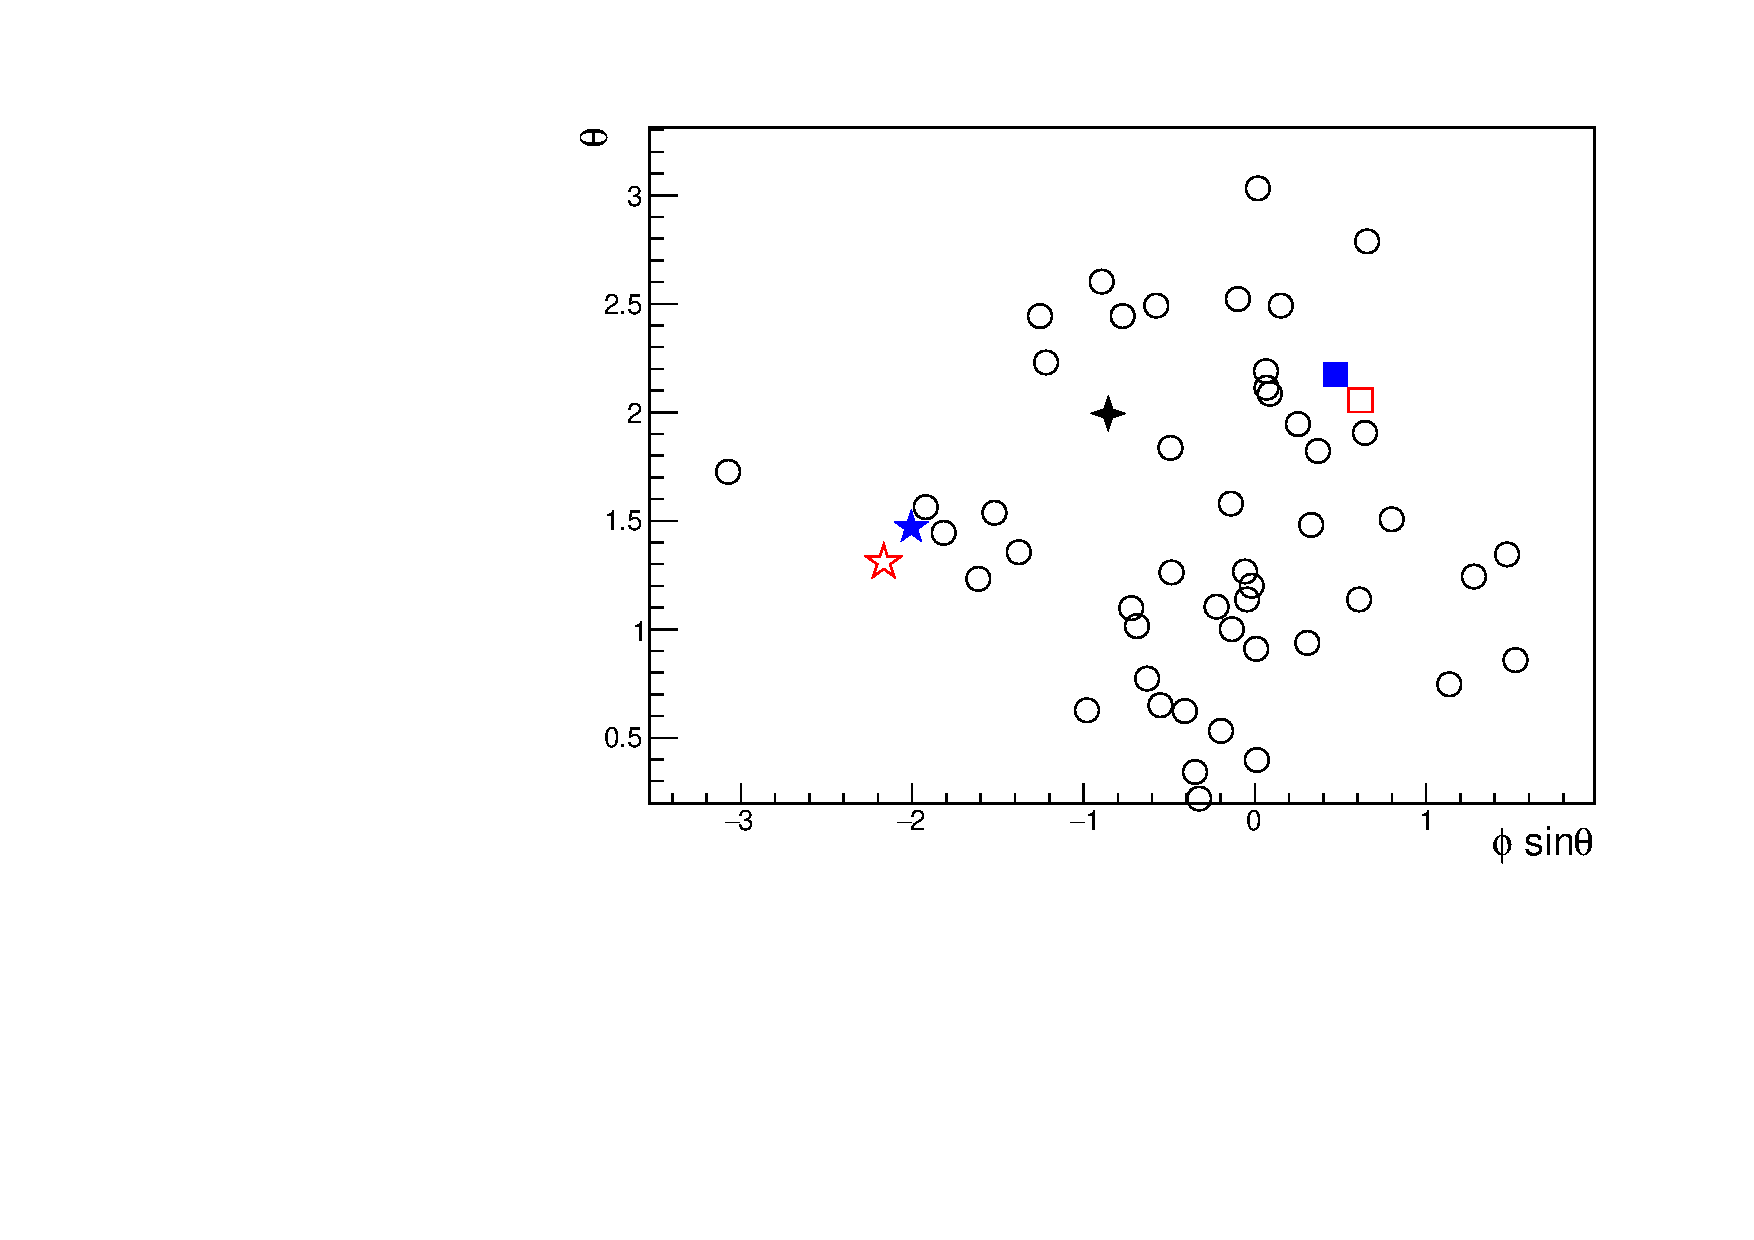
\includegraphics[width=6cm]{PMTmap_100632.pdf}
		\end{minipage}
	}
	\subfigure[Run 100663, GTID 15767175]{ 
		\begin{minipage}[t]{0.4\textwidth}
			\centering
			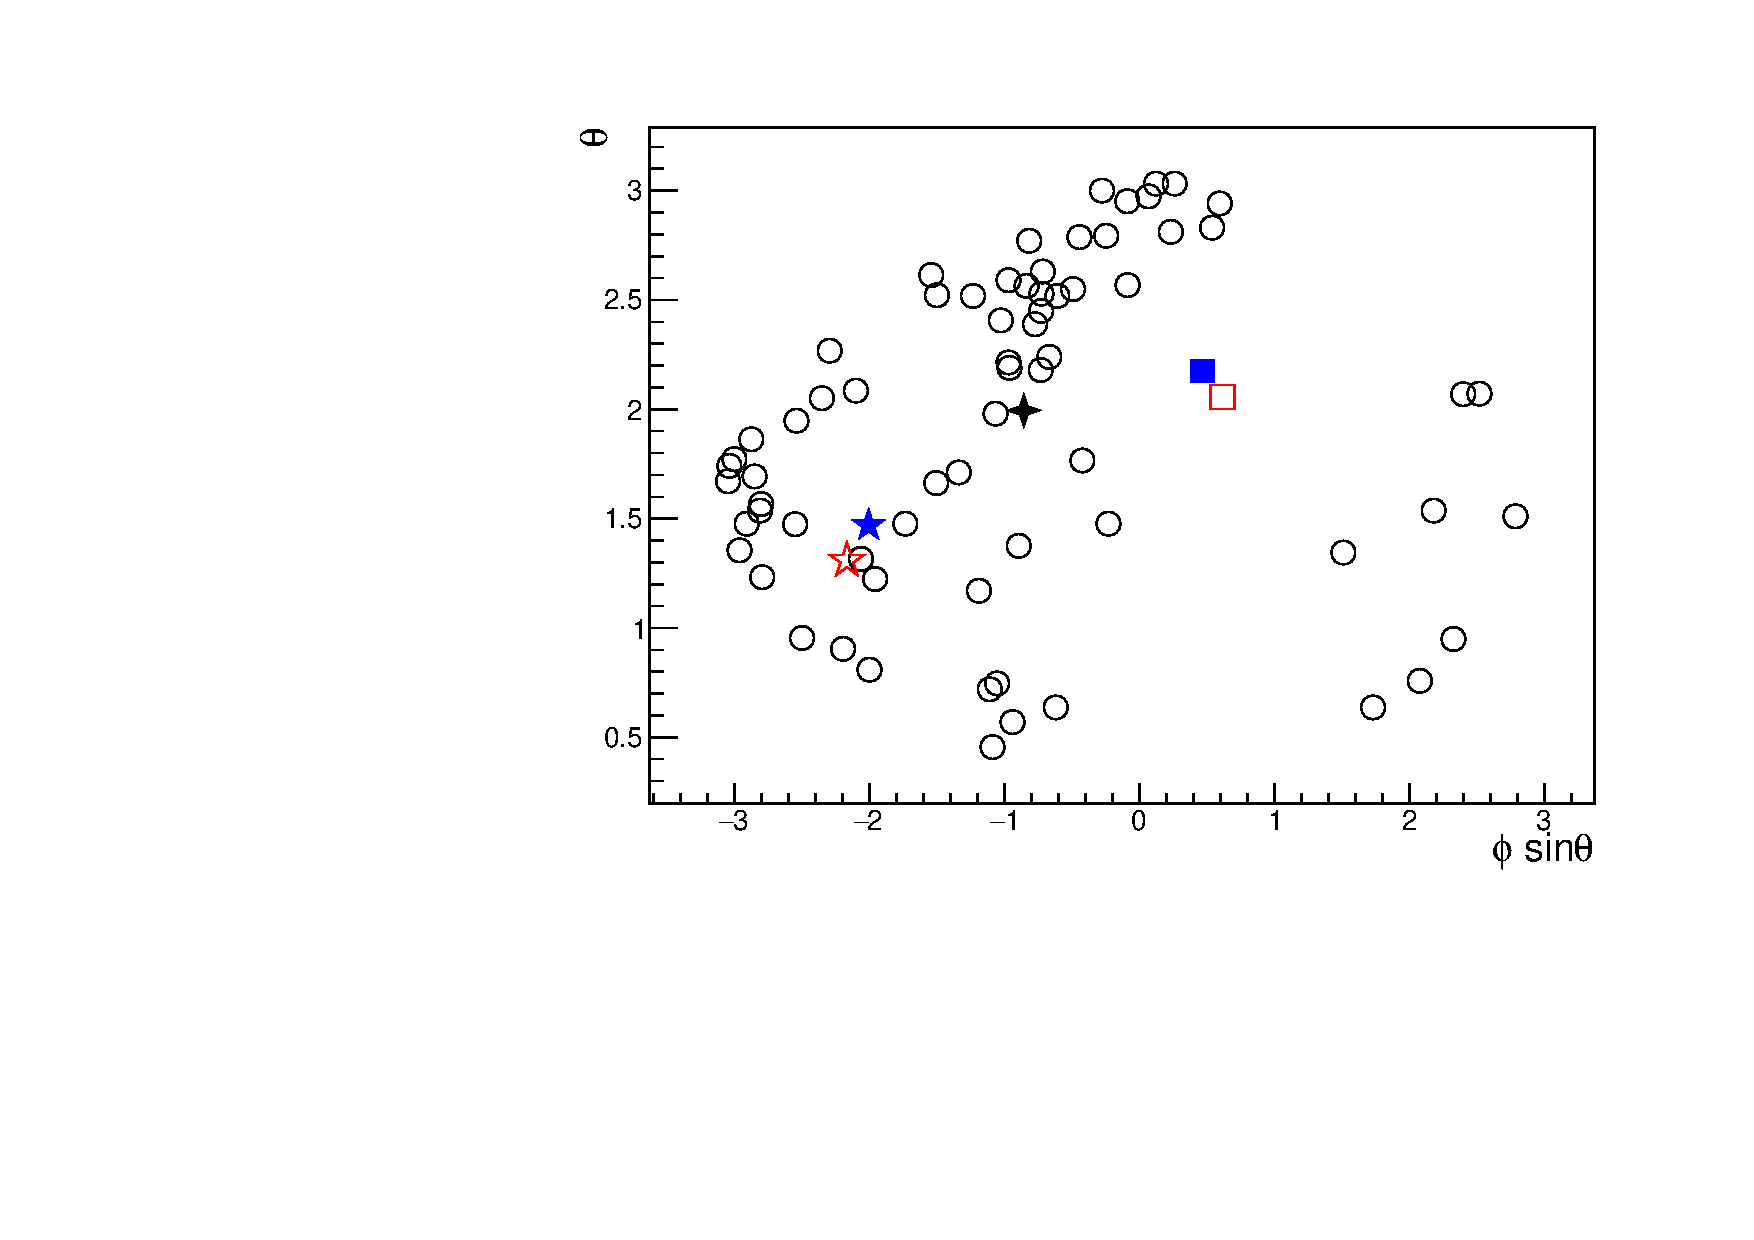
\includegraphics[width=6cm]{PMTmap_100663.pdf}
		\end{minipage}
	}
	\subfigure[Run 100915, GTID 169700]{ 
	\begin{minipage}[t]{0.4\textwidth}
		\centering
		{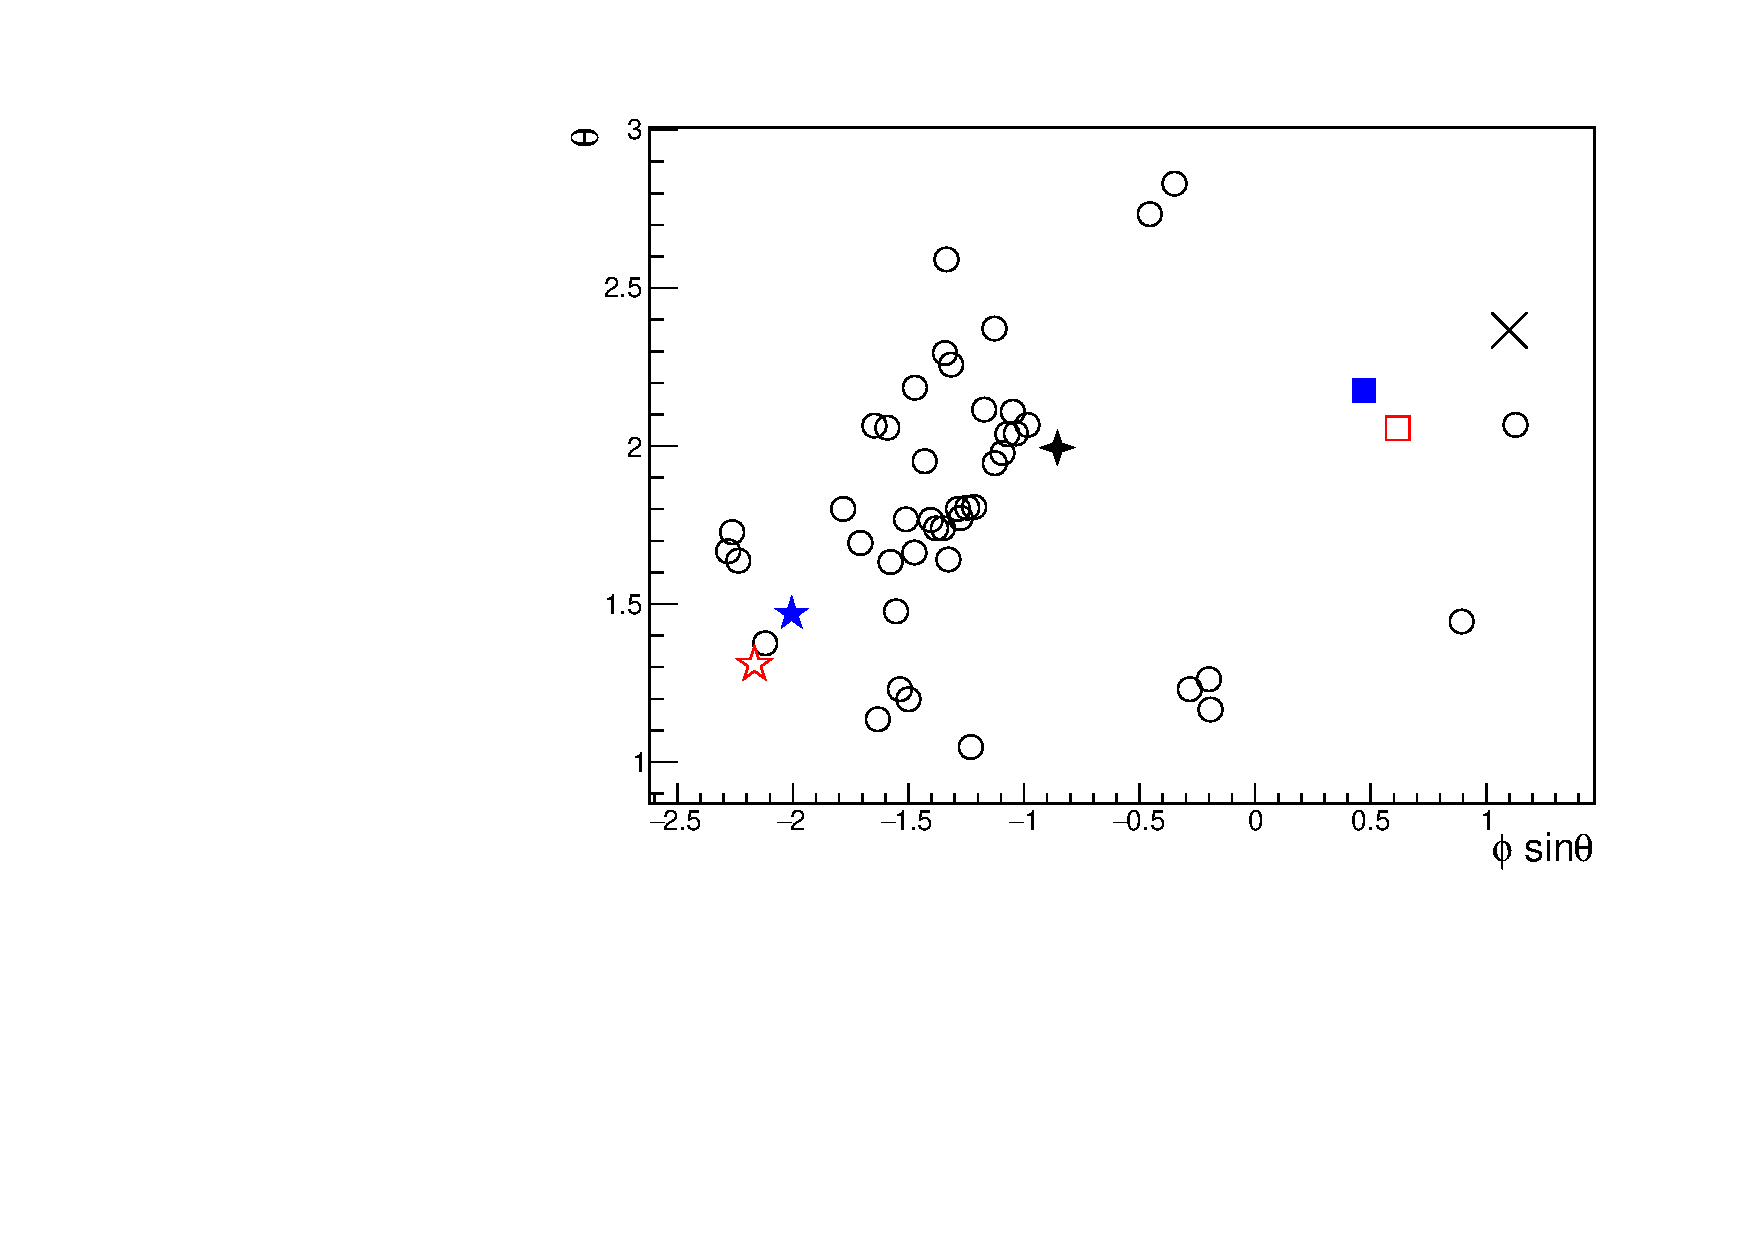
\includegraphics[width=6cm]{PMTmap_100915.pdf}}
	\end{minipage}
    }
	\subfigure[Legends]{ 
	\begin{minipage}[b]{0.4\textwidth}
		\centering
		{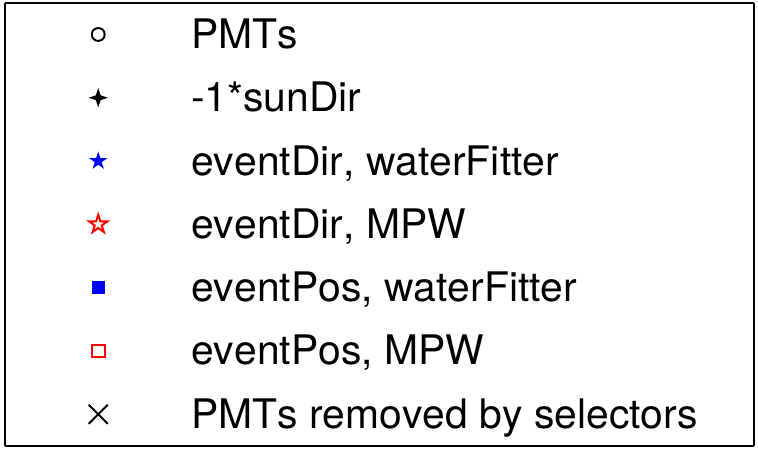
\includegraphics[width=5cm]{solarLegends.png}}
	\end{minipage}
    }
	\caption{Fit results for the candidate events, projected onto PMT sinusoidal maps. Black circles stand for
	the hit PMTs used by the fitter; crosses stand for the hit PMTs removed by the selectors; blue full star stands for the event direction fitted by the waterFitter; red open star stands for the direction fitted by the MPW; full double diamond stands for the solar direction*-1; blue full square stands for the event position fitted by the waterFitter; open square stands for the position fitted by the MPW.}
	\label{openDataSetCandidate}
\end{figure}











The Toolkit for Multivariate Data Analysis with ROOT (TMVA) \cite{tmvaWebsite}

TMVA 


other packages developed for high energy particle physics, such as StatPatternRecognition (SPR)\cite{sprWebsite}, can be considered as an alternative tool or as a reference for results comparisons. 

\subsubsection{Open Dataset Analysis}

MPW fit results


\begin{table}[ht]
	\centering
	\caption{Candidate events in the open dataset. Compared the fitted results of the candidate events with different fitters.}
	\label{opendata}
	\begin{tabular*}{150mm}{c@{\extracolsep{\fill}}cccccccc}
		\hline
	 Fitter &	Run &  GTID &  $z$(m) & $R$(m)& $(R/R_{av})^3$ & $\cos\theta_{sun}$ & SNO+ Day\\
		\hline 
	Rat & 100093 &11108354 &3.49 &3.57 &0.21 &-0.954459 &2683.92 \\	
	MPW &  --& --& 3.43 &	3.52 &	0.20	& -0.906388 & --\\
	Rat &	100207 &5079885 &-2.61 &4.60 &0.45 &0.816215 &2687.04\\
	MPW &	 --& --& -3.63 & \textbf{7.61} &	2.03 & \textbf{0.656374} & -- \\
	Rat &100632 &7882360 &1.77 &3.19 &0.15 &0.937212 &2696.93\\
	 MPW &    --& --&  1.67 & 3.11 &	0.14 & 0.910527 & -- \\
	Rat &100663 &15767175 &-4.33& 4.96 &0.56 &0.977517 &2698.18\\
	MPW & --& -- &-4.45 &	5.07 &	0.60 &	0.979943 & -- \\
	Rat &100915 &169700 &-1.00 &5.10 &0.61 &0.341287 &2701.23\\
	MPW &	--& --& -1.08 &	5.08 &	0.61 &	0.336706 & -- \\	
		\hline
	\end{tabular*}
\end{table}








